%%%%%%%%%%%%%%%%%%%%%%%%%%%%%%%%%%%%%%%%%
% Beamer Presentation
% LaTeX Template
% Version 1.0 (10/11/12)
%
% This template has been downloaded from:
% http://www.LaTeXTemplates.com
%
% License:
% CC BY-NC-SA 3.0 (http://creativecommons.org/licenses/by-nc-sa/3.0/)
%
%%%%%%%%%%%%%%%%%%%%%%%%%%%%%%%%%%%%%%%%%

%----------------------------------------------------------------------------------------
%	PACKAGES AND THEMES
%----------------------------------------------------------------------------------------

\documentclass{beamer}

\mode<presentation> {

% The Beamer class comes with a number of default slide themes
% which change the colors and layouts of slides. Below this is a list
% of all the themes, uncomment each in turn to see what they look like.

%\usetheme{default}
%\usetheme{AnnArbor}
%\usetheme{Antibes}
%\usetheme{Bergen}
%\usetheme{Berkeley}
%\usetheme{Berlin}
%\usetheme{Boadilla}
%\usetheme{CambridgeUS}
%\usetheme{Copenhagen}
%\usetheme{Darmstadt}
%\usetheme{Dresden}
%\usetheme{Frankfurt}
%\usetheme{Goettingen}
%\usetheme{Hannover}
%\usetheme{Ilmenau}
%\usetheme{JuanLesPins}
%\usetheme{Luebeck}
\usetheme{Madrid}
%\usetheme{Malmoe}
%\usetheme{Marburg}
%\usetheme{Montpellier}
%\usetheme{PaloAlto}
%\usetheme{Pittsburgh}
%\usetheme{Rochester}
%\usetheme{Singapore}
%\usetheme{Szeged}
%\usetheme{Warsaw}

% As well as themes, the Beamer class has a number of color themes
% for any slide theme. Uncomment each of these in turn to see how it
% changes the colors of your current slide theme.

%\usecolortheme{albatross}
%\usecolortheme{beaver}
%\usecolortheme{beetle}
%\usecolortheme{crane}
%\usecolortheme{dolphin}
%\usecolortheme{dove}
%\usecolortheme{fly}
%\usecolortheme{lily}
%\usecolortheme{orchid}
%\usecolortheme{rose}
%\usecolortheme{seagull}
%\usecolortheme{seahorse}
%\usecolortheme{whale}
%\usecolortheme{wolverine}

%\setbeamertemplate{footline} % To remove the footer line in all slides uncomment this line
%\setbeamertemplate{footline}[page number] % To replace the footer line in all slides with a simple slide count uncomment this line

%\setbeamertemplate{navigation symbols}{} % To remove the navigation symbols from the bottom of all slides uncomment this line
}

\usepackage{graphicx} % Allows including images
\usepackage{booktabs} % Allows the use of \toprule, \midrule and \bottomrule in tables

%----------------------------------------------------------------------------------------
%	TITLE PAGE
%----------------------------------------------------------------------------------------

\title[Similarity Measures]{Evaluation of semantic similarity measures} % The short title appears at the bottom of every slide, the full title is only on the title page

\author{Maxat Kulmanov} % Your name
\institute[KAUST, CBRC] % Your institution as it will appear on the bottom of every slide, may be shorthand to save space
{
King Abdullah University of Science and Technology \\ % Your institution for the title page
\medskip
% \textit{maxat.kulmanov@kaust.edu.sa} % Your email address
}
\date{\today} % Date, can be changed to a custom date

\begin{document}

\begin{frame}
\titlepage % Print the title page as the first slide
\end{frame}

\begin{frame}
\frametitle{Overview} % Table of contents slide, comment this block out to remove it
\tableofcontents % Throughout your presentation, if you choose to use \section{} and \subsection{} commands, these will automatically be printed on this slide as an overview of your presentation
\end{frame}

%----------------------------------------------------------------------------------------
%	PRESENTATION SLIDES
%----------------------------------------------------------------------------------------

%------------------------------------------------
\section{Introduction} % Sections can be created in order to organize your presentation into discrete blocks, all sections and subsections are automatically printed in the table of contents as an overview of the talk
%------------------------------------------------

%\subsection{Subsection Example} % A subsection can be created just before a set of slides with a common theme to further break down your presentation into chunks

\begin{frame}
\frametitle{Semantic Similarity Measures}
\begin{itemize}
\item Semantic similarity measures capture the strength of interaction between concepts based on their meaning \cite{p1}.
\item Based on text corpus or ontologies
\end{itemize}
\end{frame}

%------------------------------------------------

\section{Problem definition}

\begin{frame}
\frametitle{Problem definition}
\begin{itemize}
\item Large number of semantic similarity measures
\item Which one to choose?
\end{itemize}
\end{frame}

%------------------------------------------------

\section{Project aim}

\begin{frame}
\frametitle{Project aim}
\begin{itemize}
\item Analyze similarity measure dependence on the number of classes
\item Analyze similarity measure dependence on the difference of the number of classes
\item Analyze similarity measure dependence on the depth of classes
\end{itemize}
\end{frame}

%------------------------------------------------

\section{Datasets}

%------------------------------------------------

\begin{frame}
\frametitle{Datasets}
\begin{itemize}
\item Gene Ontology
\item Yeast Genome Database annotations
\item 5500 Randomly generated annotations with size from 1 to 55 for each 100
\item 1700 Randomly generated annotations with depth from 1 to 17
\end{itemize}
\end{frame}
%------------------------------------------------



\section{List of similarity measures}
%------------------------------------------------

\begin{frame}
\frametitle{Groupwise similarity measures}
\begin{table}
\begin{tabular}{l l}
\toprule
\textbf{Direct groupwise measures} \\
\midrule
SOKAL, SNEATH 1963 & BADER 2003 \\
TVERSKY 1977 & BATET 2010 \\
ALI, DEANE & BRAUN, BLANQUET 1932 \\
GIC (Graph Information Content) & DICE 1945 \\
LEE 2004 & JACCARD 1901 \\
LP (Longest shared path) & KNAPPE 2004 \\
NTO (Normalized Term Overlap) & KORBEL 2002 \\
NTO MAX & MARYLAND, BRIDGE 2003 \\
TO (Term Overlap) & OCHIAI 1957 \\
UI (Union Intersection) & SIMPSON 1960 \\
SVM &  \\

\bottomrule
\end{tabular}
\caption{Direct groupwise similarity measures}
\end{table}
\end{frame}

%------------------------------------------------

\begin{frame}
\frametitle{Pairwise similarity measures}
\begin{table}
\resizebox{\textwidth}{!}{%
\begin{tabular}{l l}
\toprule
\textbf{Edge and node based pairwise measures} \\
\midrule
KYOGOKU BASIC 2011 & LEACOCK CHODOROW 1998 \\ 
LI 2003 & PEKAR STAAB 2002 \\
RADA 1989 & RADA LCA 1989 \\
RESNIK 1995 & SLIMANI 2006 \\
STOJANOVIC 2001 & WU PALMER 1994 \\
HYBRID RANWEZ 2006 & FEATURE TVERSKY CONTRAST MODEL \\
FEATURE TVERSKY RATIO MODEL & GL \\ 
GL GRASM & HARISPE 2013 \\
JACCARD 3W IC & JACCARD IC \\ 
JIANG CONRATH 1997 & JIANG CONRATH 1997 NORM \\
LIN 1998 & LIN 1998 GraSM \\
MAZANDU 2012 & RESNIK 1995 \\
RESNIK 1995 ANCESTORS & RESNIK 1995 DESCENDANTS \\ 
RESNIK 1995 GraSM & SCHLICKER 2006 \\
SCHLICKER 3WJACCARD & SCHLICKER GL \\ 
SCHLICKER JACCARD & SCHLICKER TVERSKY \\
SIM IC 2010 & TVERSKY IC CONTRAST MODEL \\
TVERSKY IC PROP CONTRAST MODEL & TVERSKY IC PROP RATIO MODEL \\
TVERSKY IC RATIO MODEL & RANDOM \\
\bottomrule
\end{tabular}}
\caption{Pairwise similarity measures}
\end{table}
\end{frame}

%------------------------------------------------

\begin{frame}
\frametitle{Pairwise similarity measures}
\begin{table}
\begin{tabular}{|l|}
\toprule
\textbf{Indirect groupwise measures} \\
\midrule
Average \\
Average Normilized GoSim \\
Best Match Average \\
Best Match Max \\
Max \\
Min \\
Max Normalized GoSim \\
\bottomrule
\end{tabular}
\caption{Indirect groupwise similarity measures}
\end{table}
\end{frame}

%------------------------------------------------
\section{Methods}

\begin{frame}
\frametitle{Methods}
\begin{itemize}
\item Semantic measures library \cite{p2}
\item Spearman Correlation coefficient
\item Pearson Correlation coefficient
\end{itemize}
\end{frame}

%------------------------------------------------

\section{Results}

\begin{frame}
\frametitle{Results}
\begin{itemize}
\item Classification of the similarity measures based on sensitivity to: 
\begin{itemize}
	\item Number of classes
    \item Difference of number of classes
    \item Depth of classes
\end{itemize}
\end{itemize}
\end{frame}

\begin{frame}{Groupwise Similarity Measures}

\begin{figure}
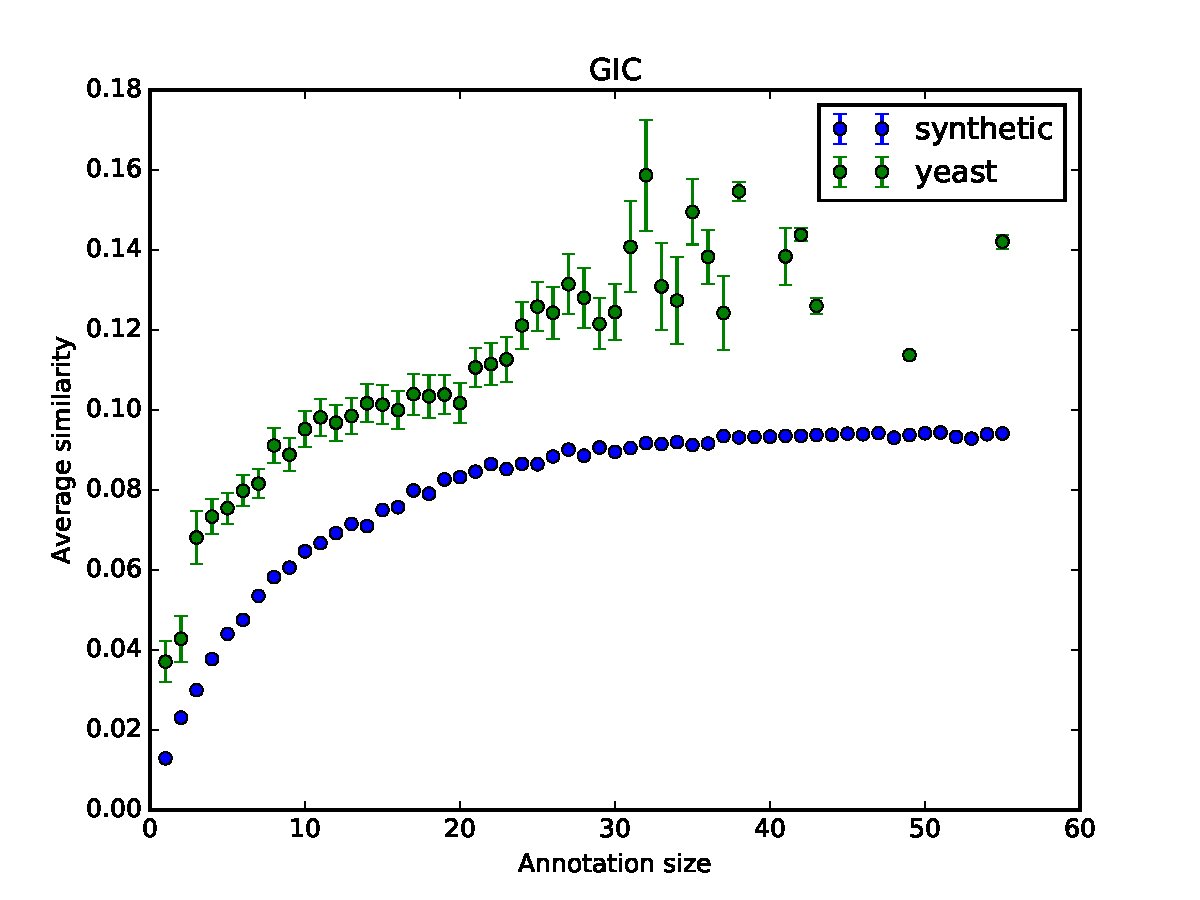
\includegraphics[width=0.5\linewidth, height=0.4\textheight]{groupwise/SIM_GROUPWISE_DAG_GIC_avg.pdf}
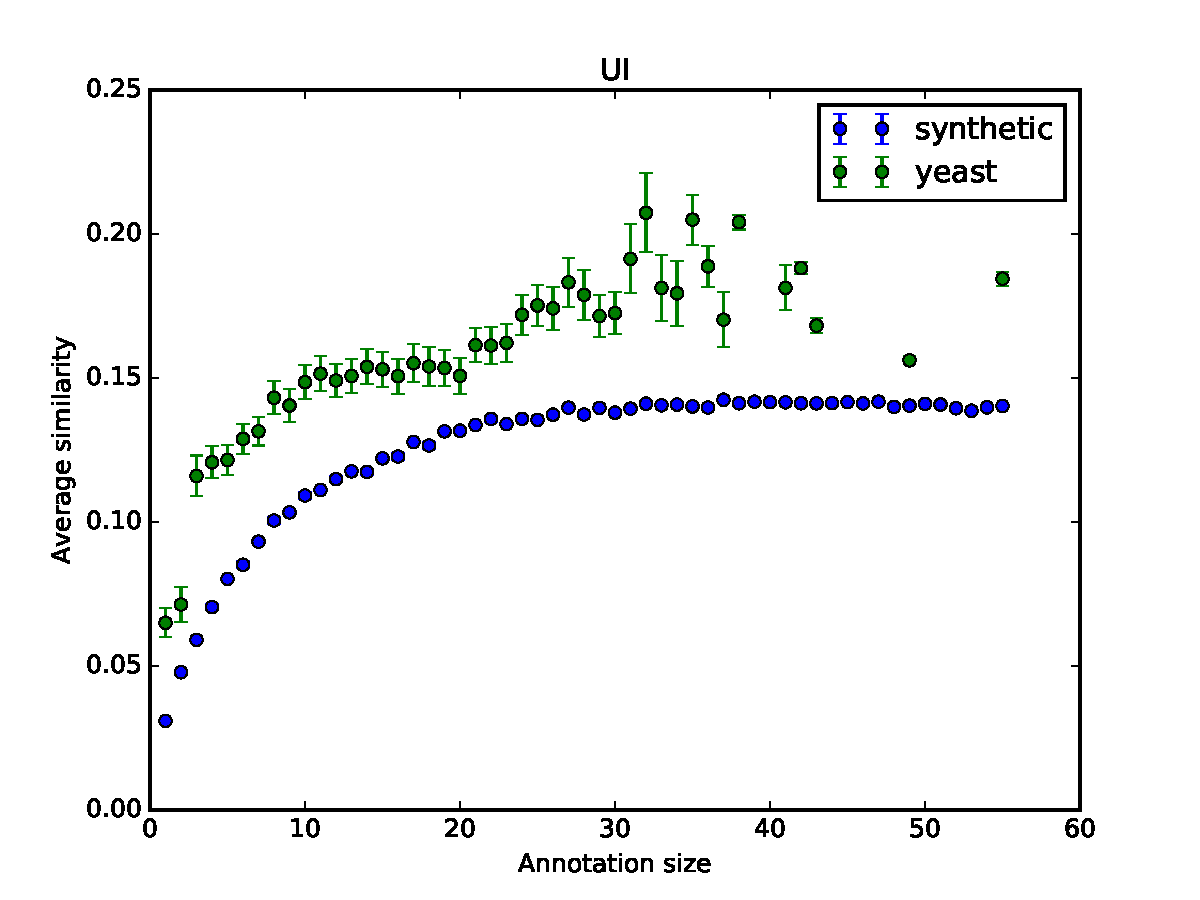
\includegraphics[width=0.5\linewidth, height=0.4\textheight]{groupwise/SIM_GROUPWISE_DAG_UI_avg.pdf} \\
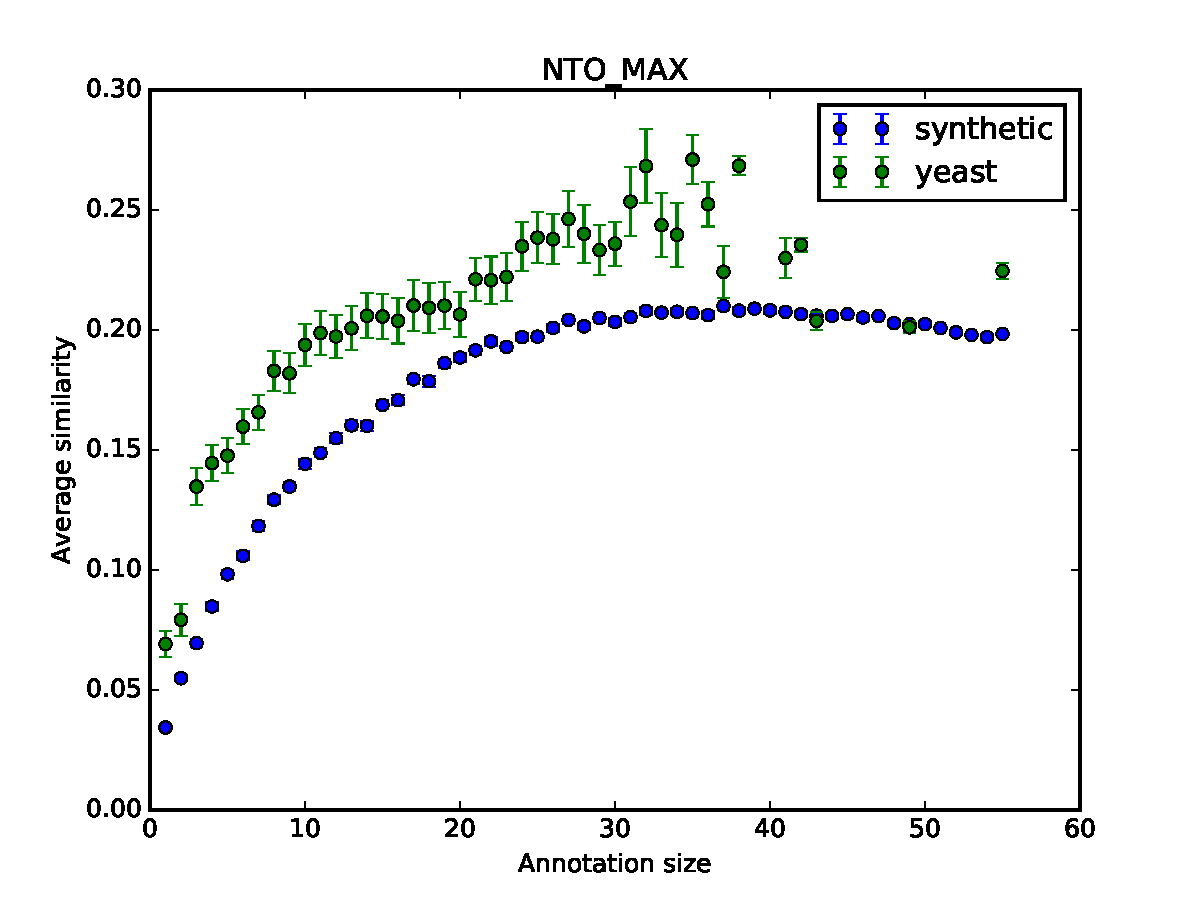
\includegraphics[width=0.5\linewidth, height=0.4\textheight]{groupwise/SIM_GROUPWISE_DAG_NTO_MAX_avg.pdf}
\end{figure}

\end{frame}

\begin{frame}{Groupwise Similarity Measures}

\begin{figure}
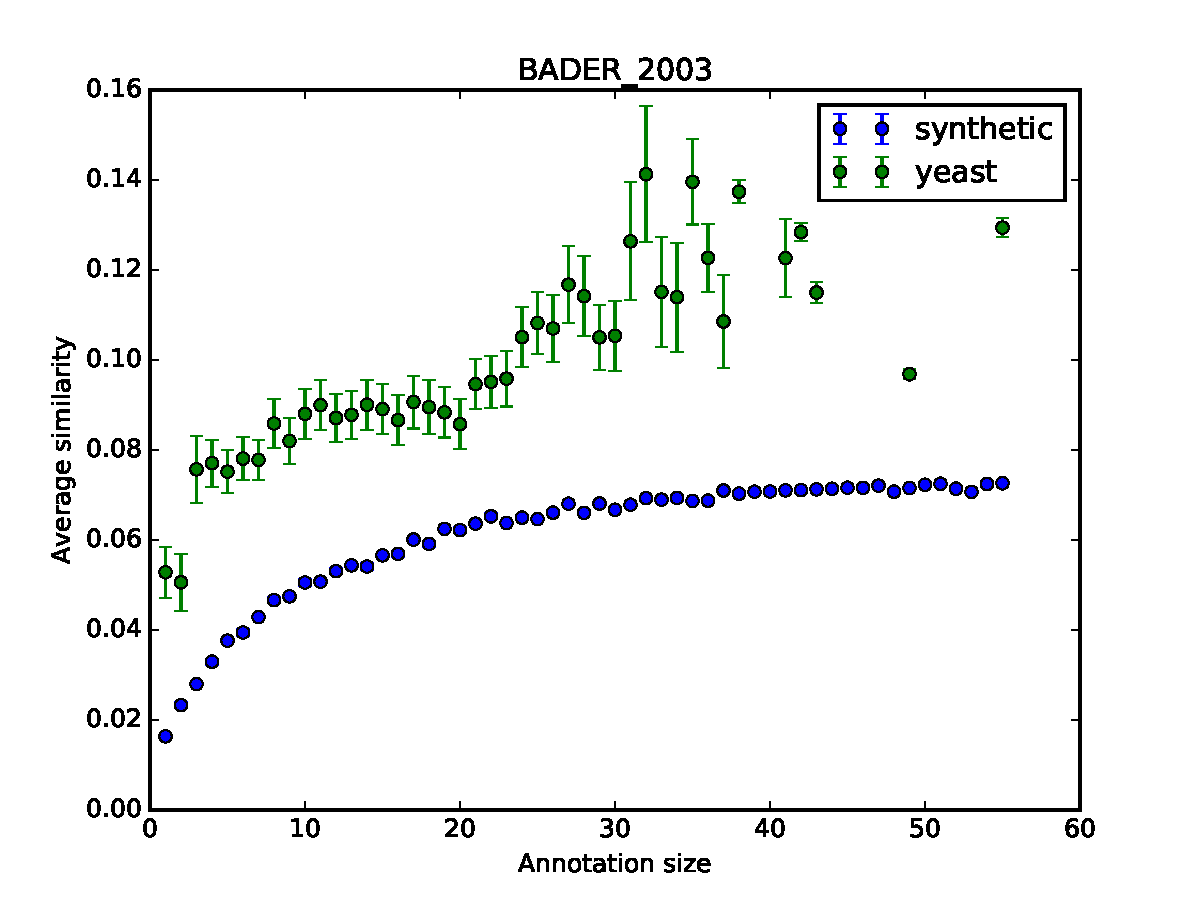
\includegraphics[width=0.5\linewidth, height=0.4\textheight]{groupwise/SIM_FRAMEWORK_DAG_SET_BADER_2003_avg.pdf}
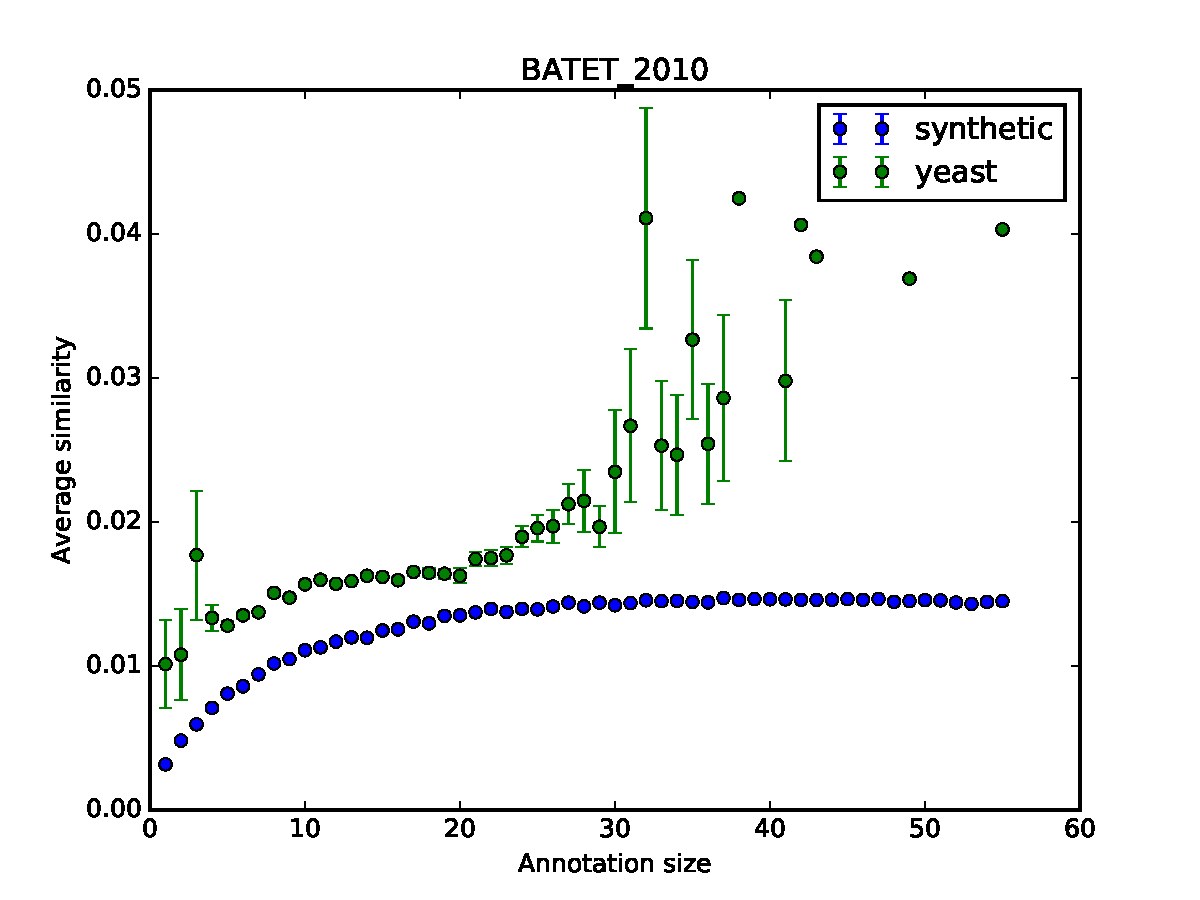
\includegraphics[width=0.5\linewidth, height=0.4\textheight]{groupwise/SIM_FRAMEWORK_DAG_SET_BATET_2010_avg.pdf} \\
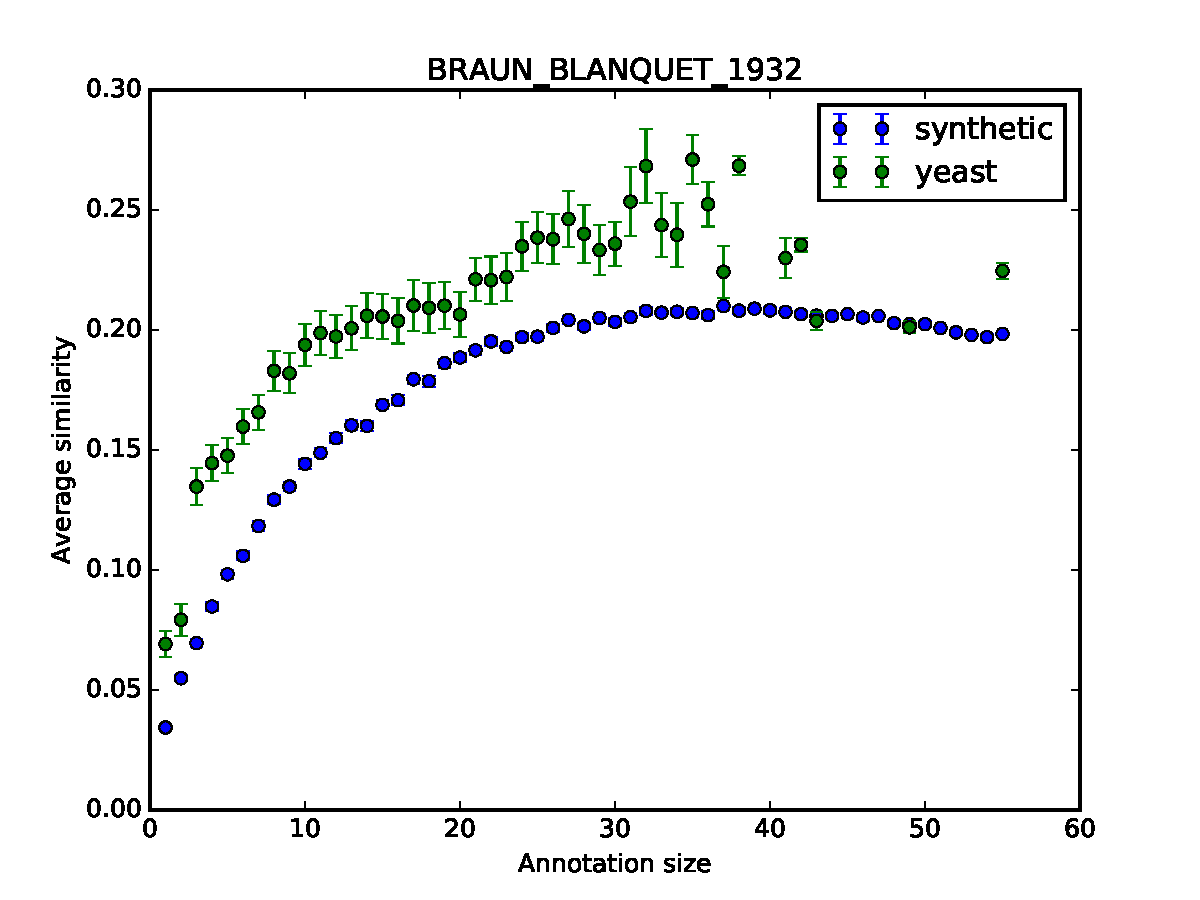
\includegraphics[width=0.5\linewidth, height=0.4\textheight]{groupwise/SIM_FRAMEWORK_DAG_SET_BRAUN_BLANQUET_1932_avg.pdf}
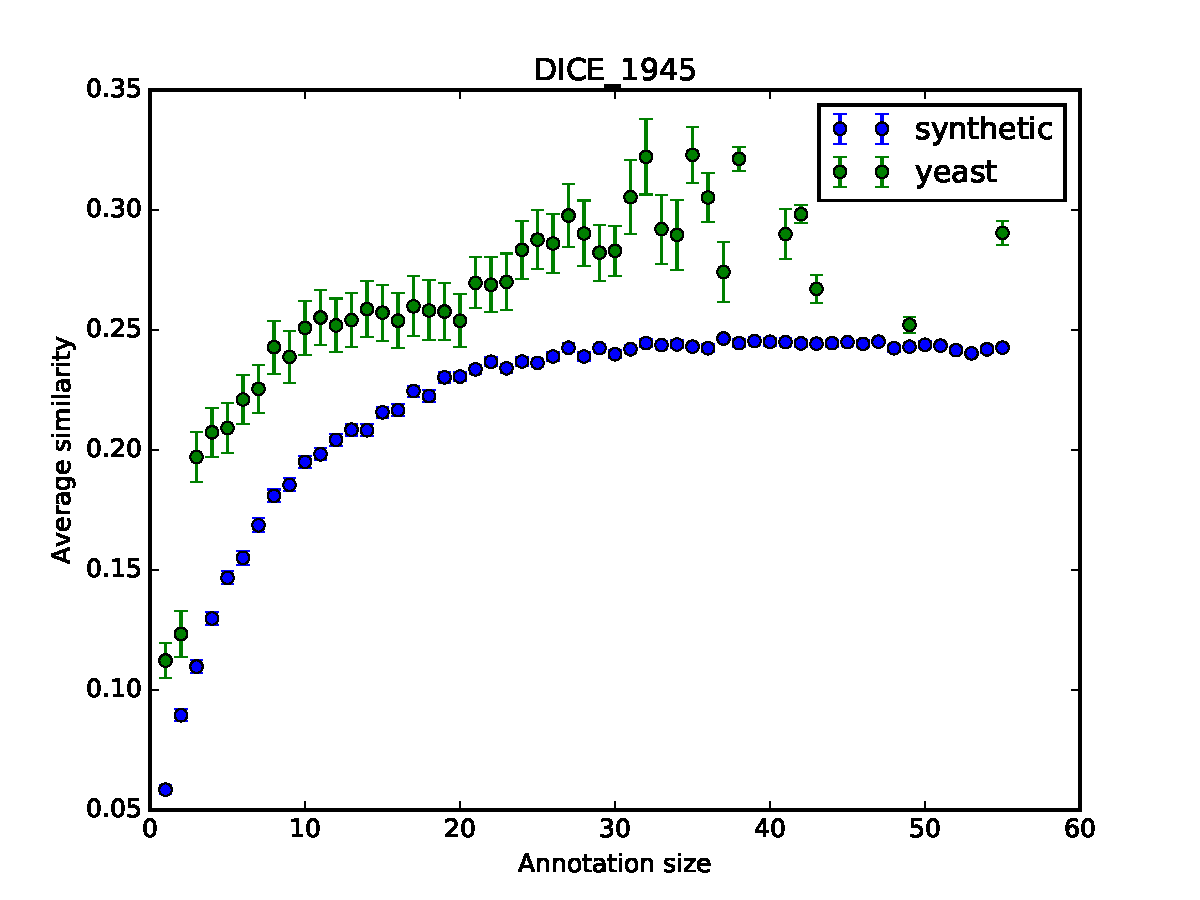
\includegraphics[width=0.5\linewidth, height=0.4\textheight]{groupwise/SIM_FRAMEWORK_DAG_SET_DICE_1945_avg.pdf}
\end{figure}

\end{frame}

\begin{frame}{Groupwise Similarity Measures}

\begin{figure}
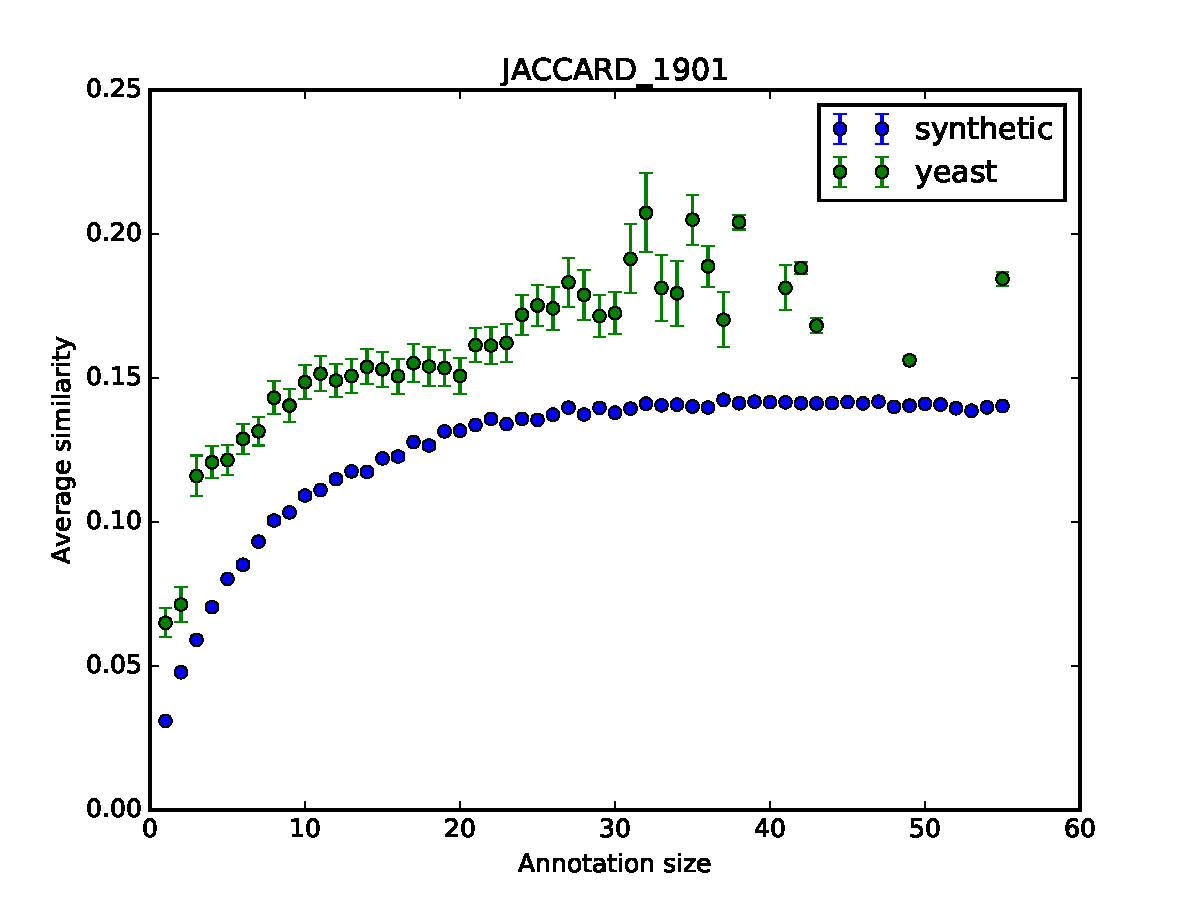
\includegraphics[width=0.5\linewidth, height=0.4\textheight]{groupwise/SIM_FRAMEWORK_DAG_SET_JACCARD_1901_avg.pdf}
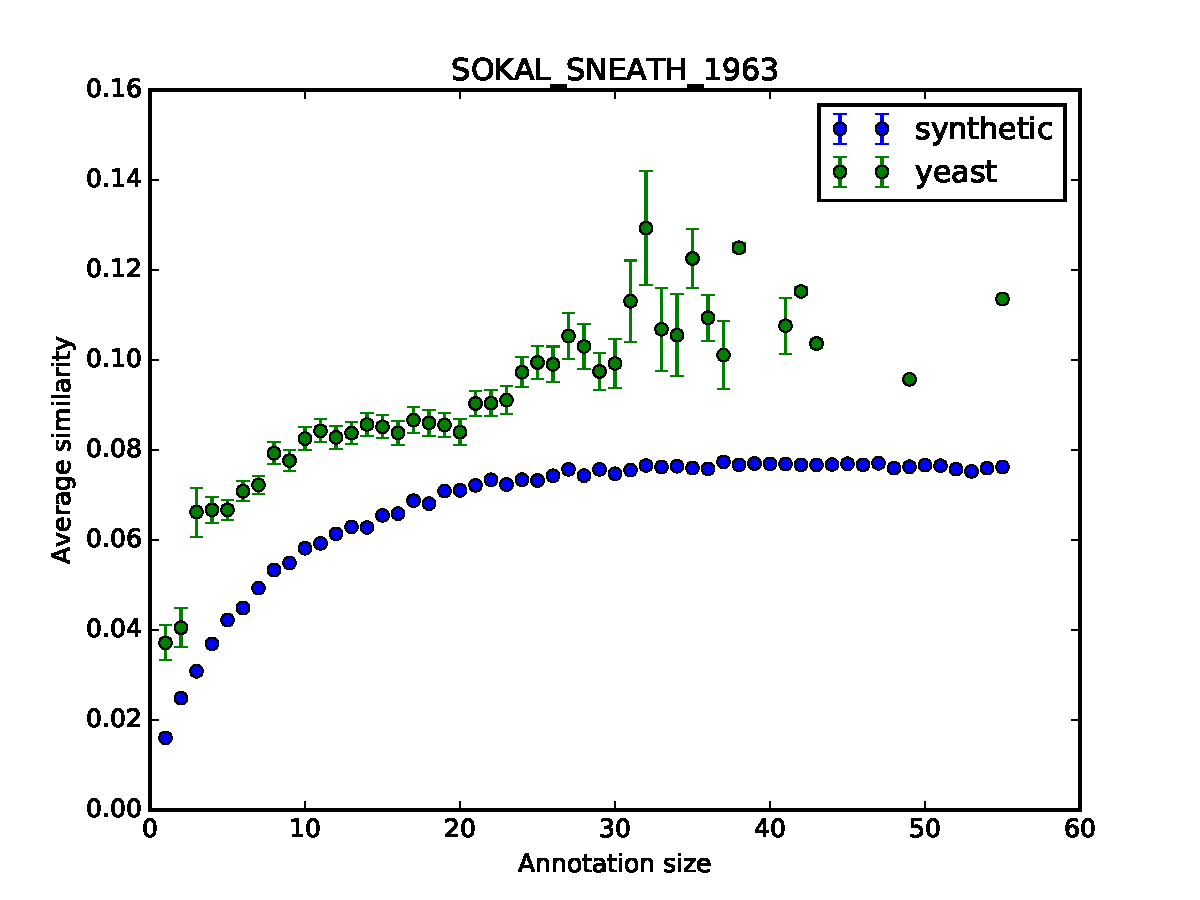
\includegraphics[width=0.5\linewidth, height=0.4\textheight]{groupwise/SIM_FRAMEWORK_DAG_SET_SOKAL_SNEATH_1963_avg.pdf} \\
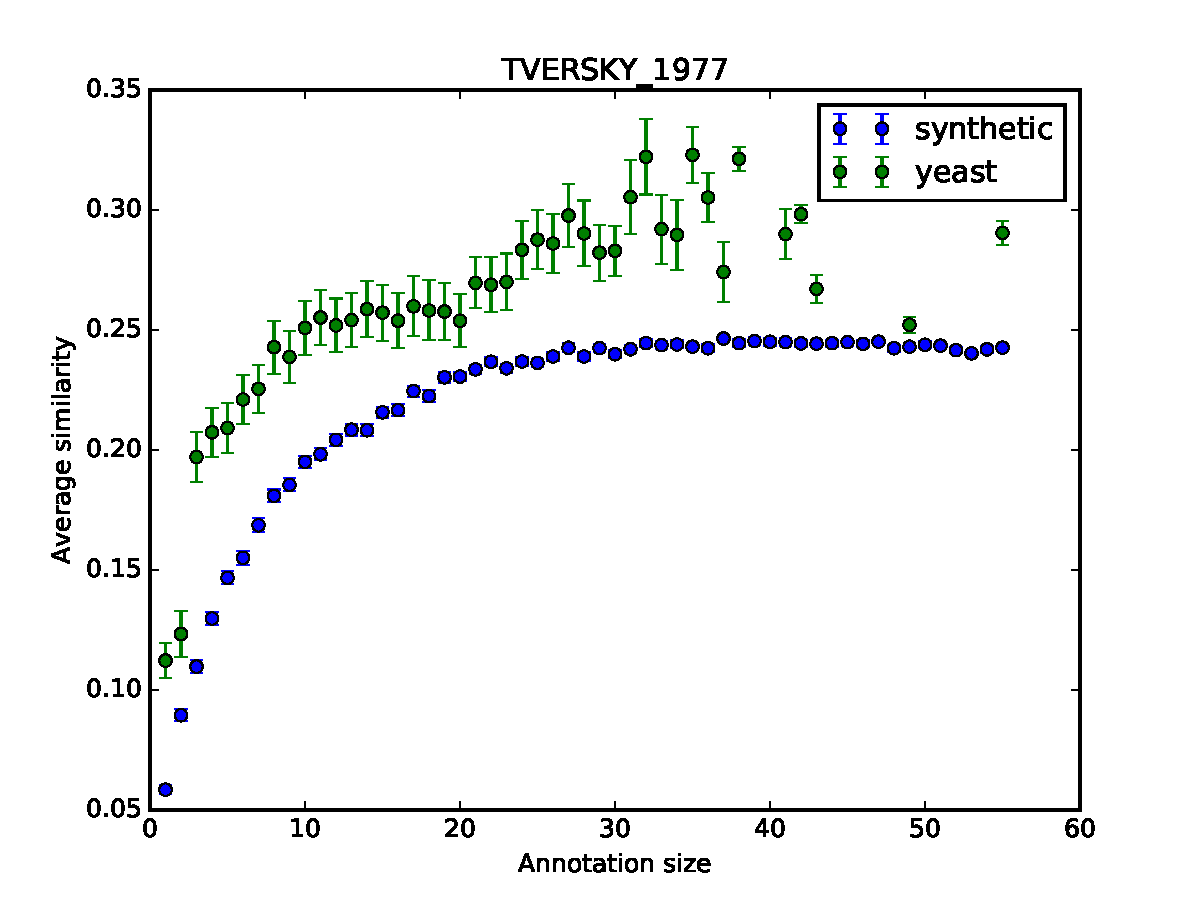
\includegraphics[width=0.5\linewidth, height=0.4\textheight]{groupwise/SIM_FRAMEWORK_DAG_SET_TVERSKY_1977_avg.pdf}
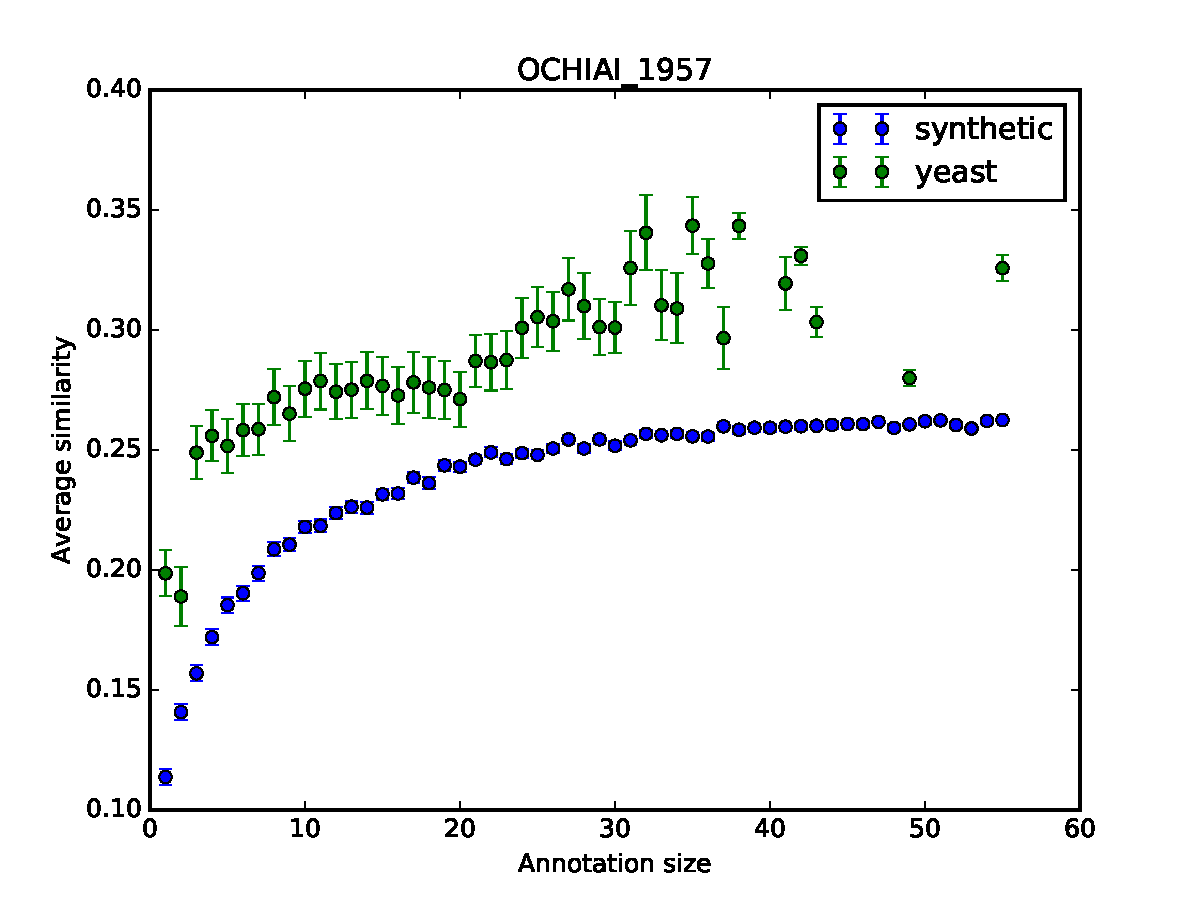
\includegraphics[width=0.5\linewidth, height=0.4\textheight]{groupwise/SIM_FRAMEWORK_DAG_SET_OCHIAI_1957_avg.pdf}
\end{figure}

\end{frame}

\begin{frame}{Groupwise Similarity Measures}

\begin{figure}
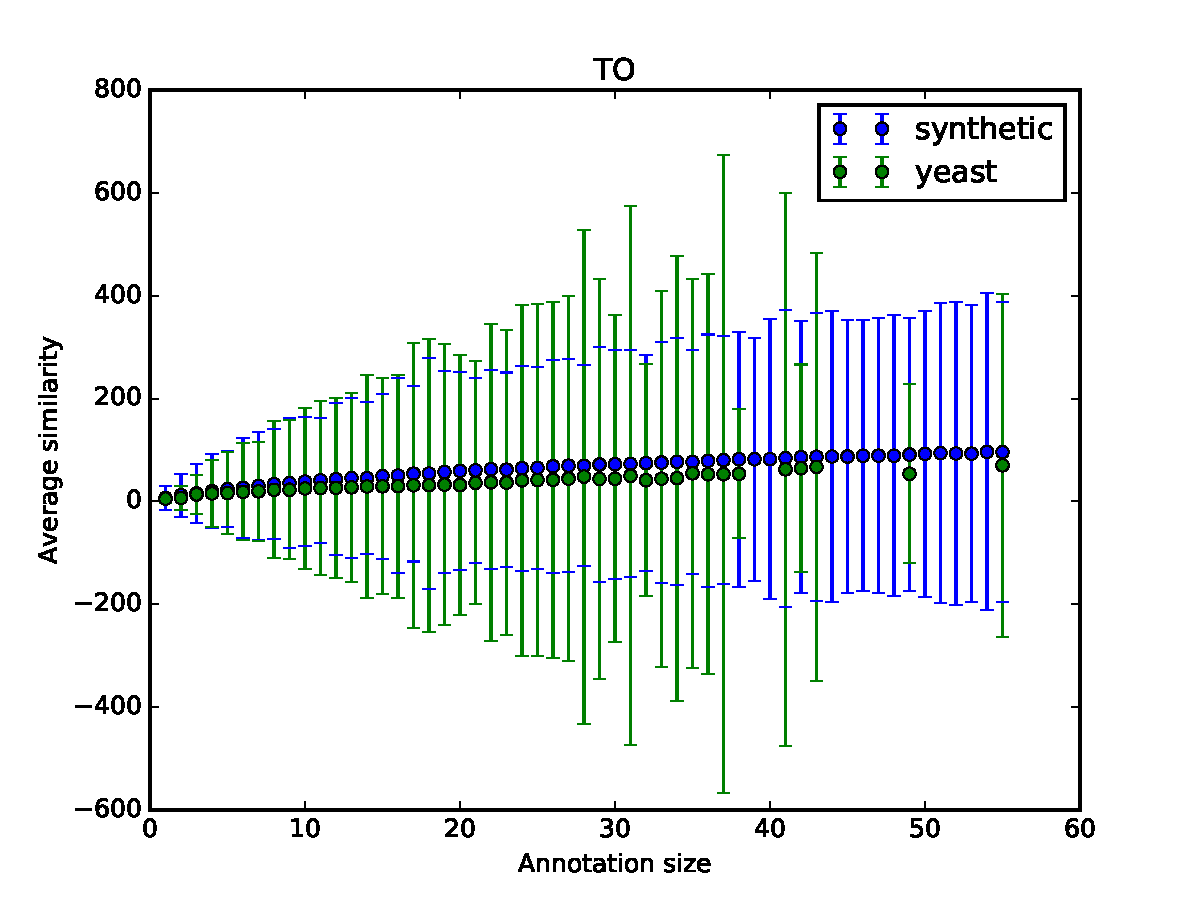
\includegraphics[width=0.5\linewidth, height=0.4\textheight]{groupwise/SIM_GROUPWISE_DAG_TO_avg.pdf}
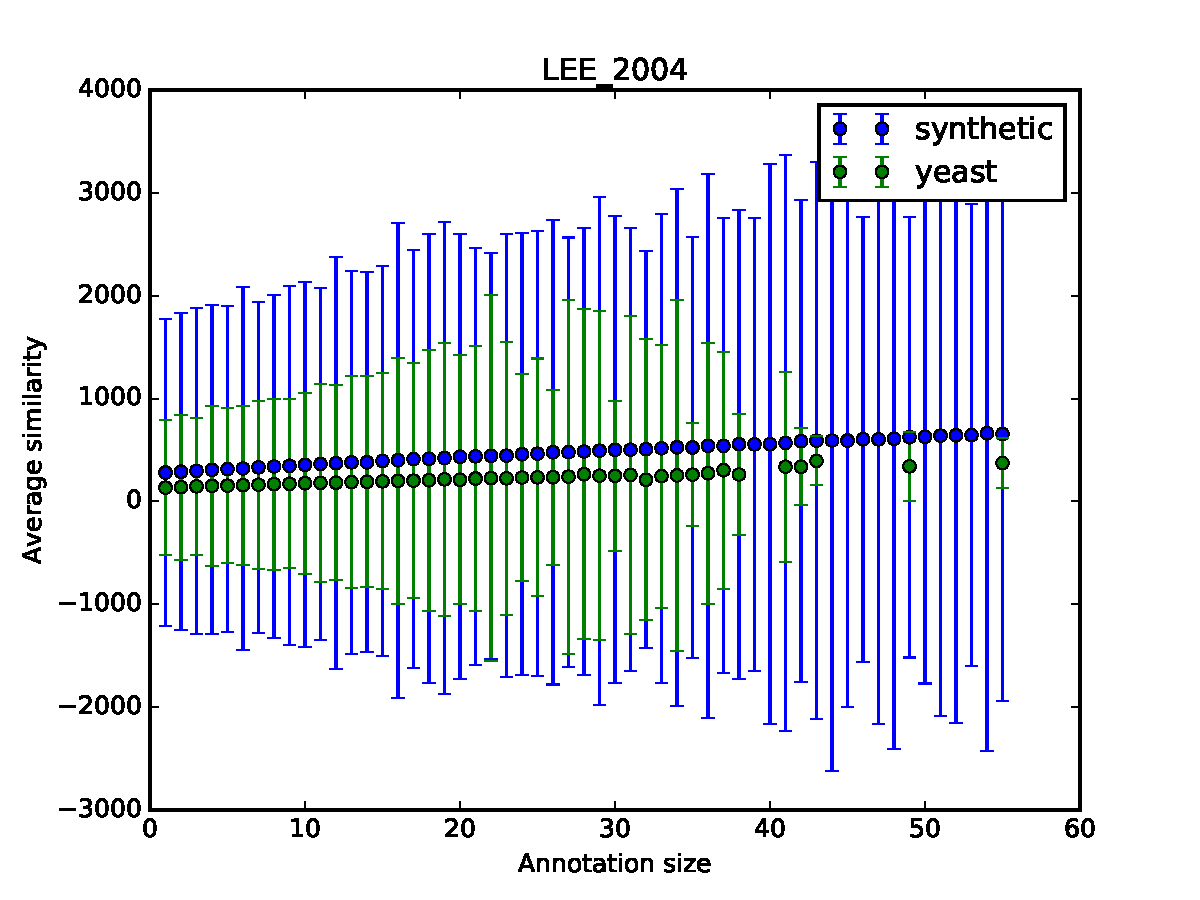
\includegraphics[width=0.5\linewidth, height=0.4\textheight]{groupwise/SIM_GROUPWISE_DAG_LEE_2004_avg.pdf} \\
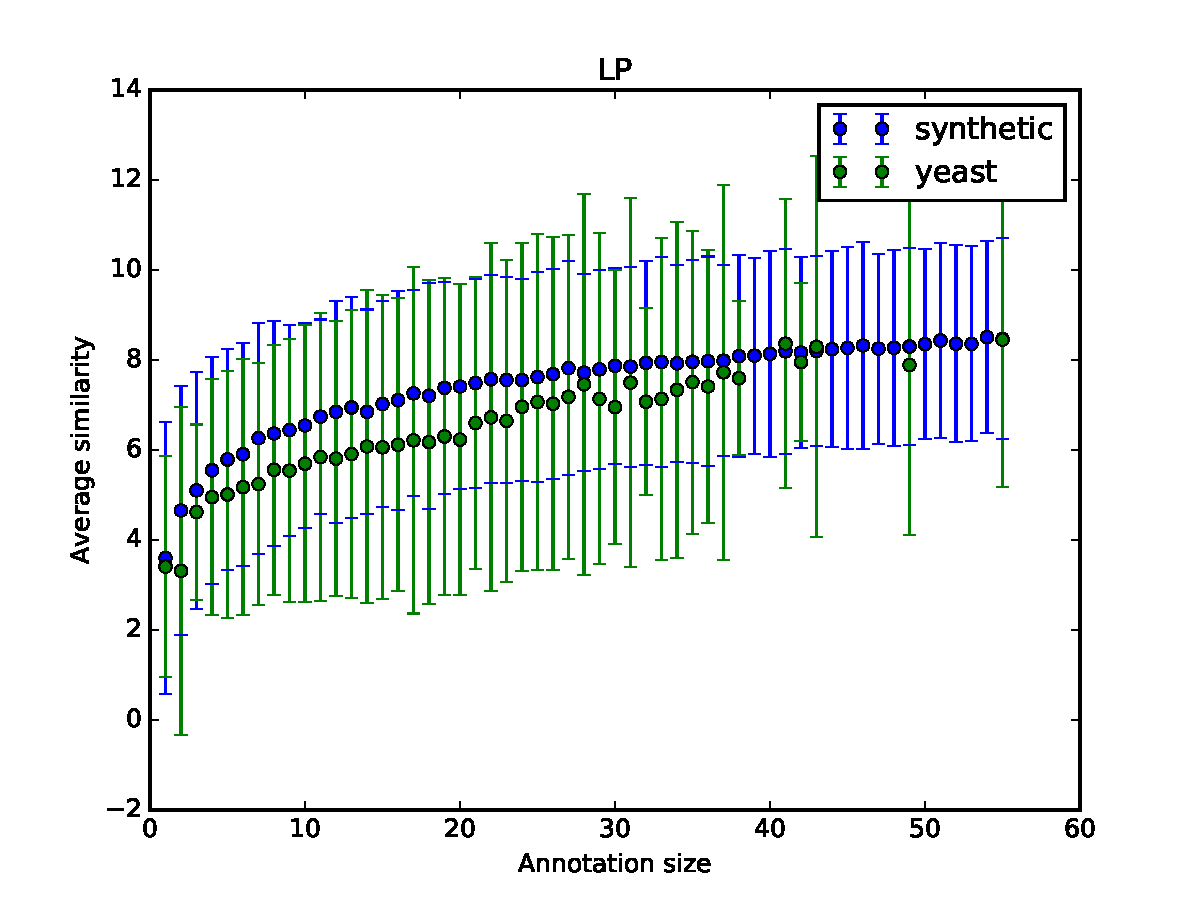
\includegraphics[width=0.5\linewidth, height=0.4\textheight]{groupwise/SIM_GROUPWISE_DAG_LP_avg.pdf}
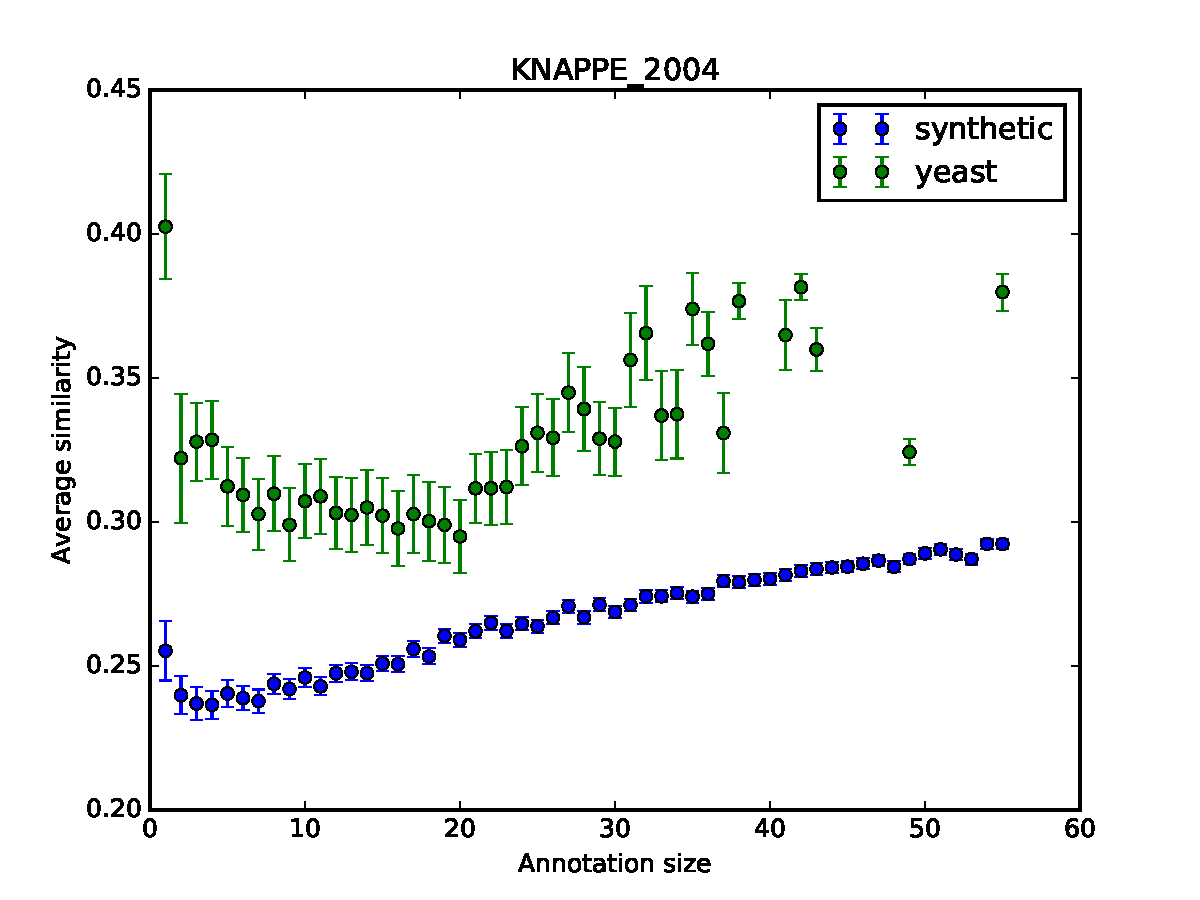
\includegraphics[width=0.5\linewidth, height=0.4\textheight]{groupwise/SIM_FRAMEWORK_DAG_SET_KNAPPE_2004_avg.pdf}
\end{figure}

\end{frame}

\begin{frame}{Groupwise Similarity Measures}

\begin{figure}
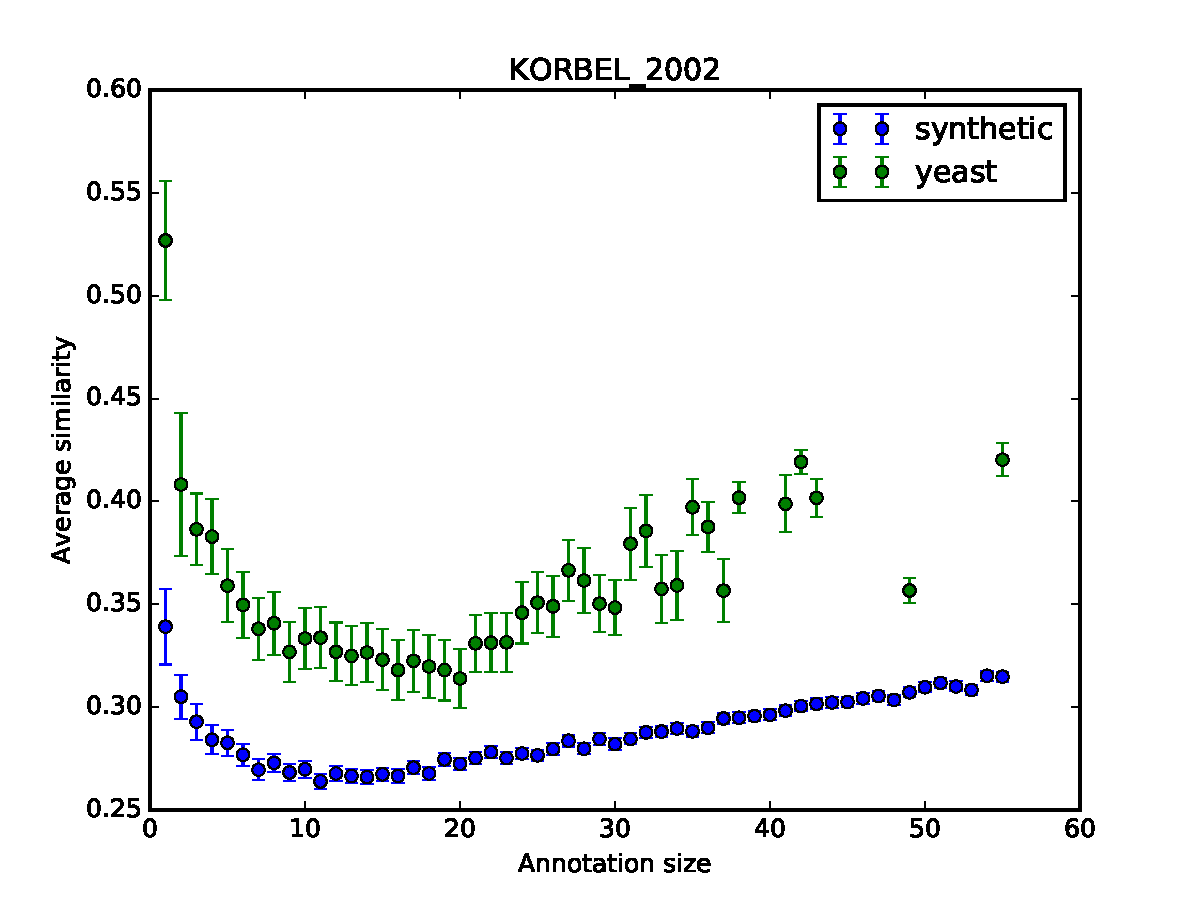
\includegraphics[width=0.5\linewidth, height=0.4\textheight]{groupwise/SIM_FRAMEWORK_DAG_SET_KORBEL_2002_avg.pdf}
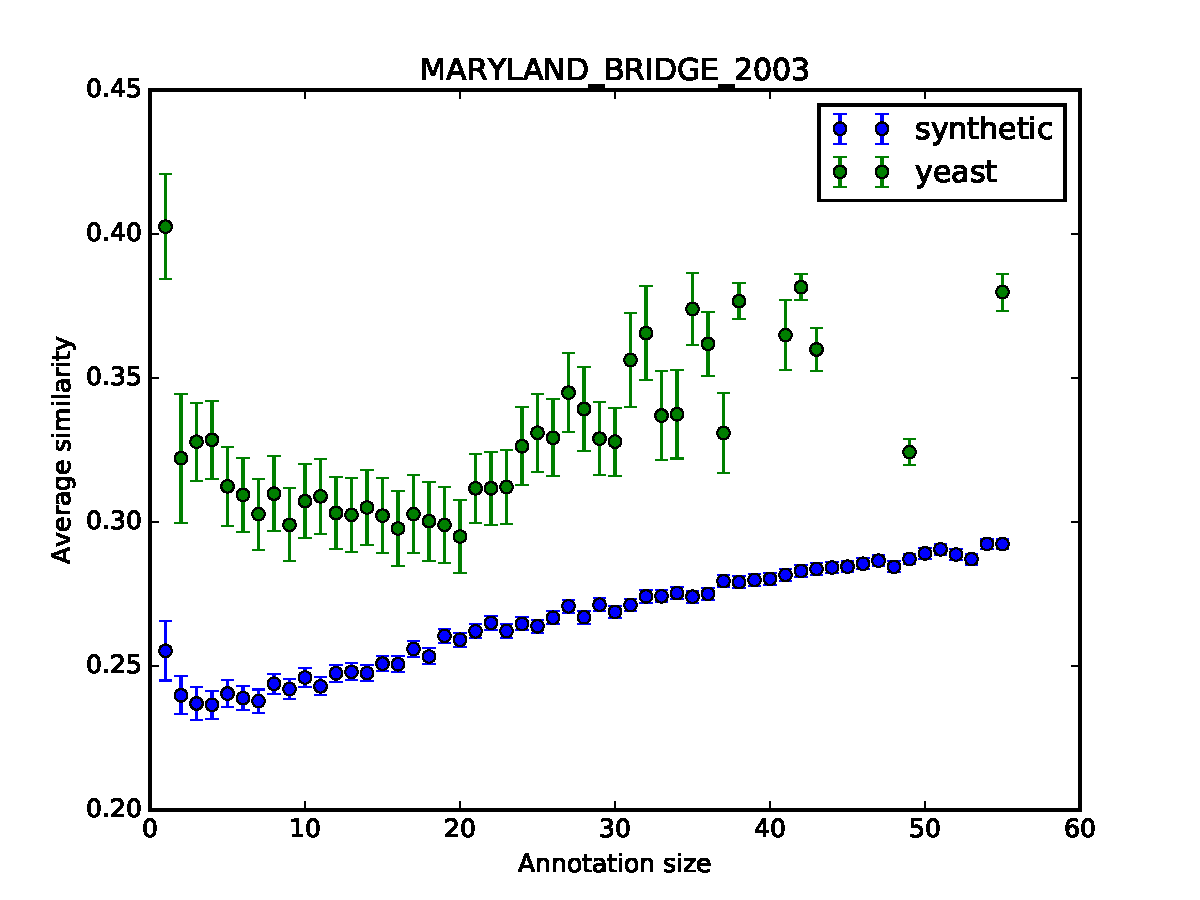
\includegraphics[width=0.5\linewidth, height=0.4\textheight]{groupwise/SIM_FRAMEWORK_DAG_SET_MARYLAND_BRIDGE_2003_avg.pdf} \\
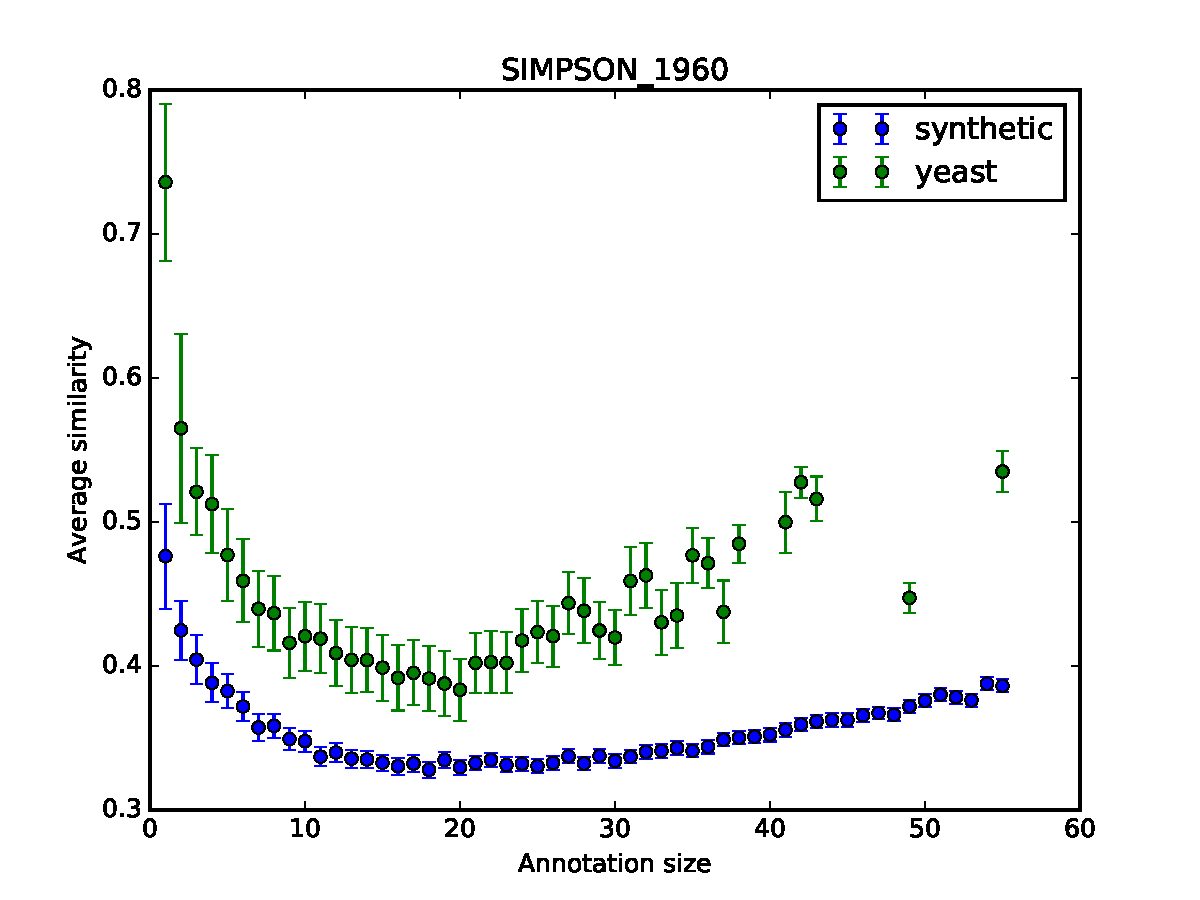
\includegraphics[width=0.5\linewidth, height=0.4\textheight]{groupwise/SIM_FRAMEWORK_DAG_SET_SIMPSON_1960_avg.pdf}
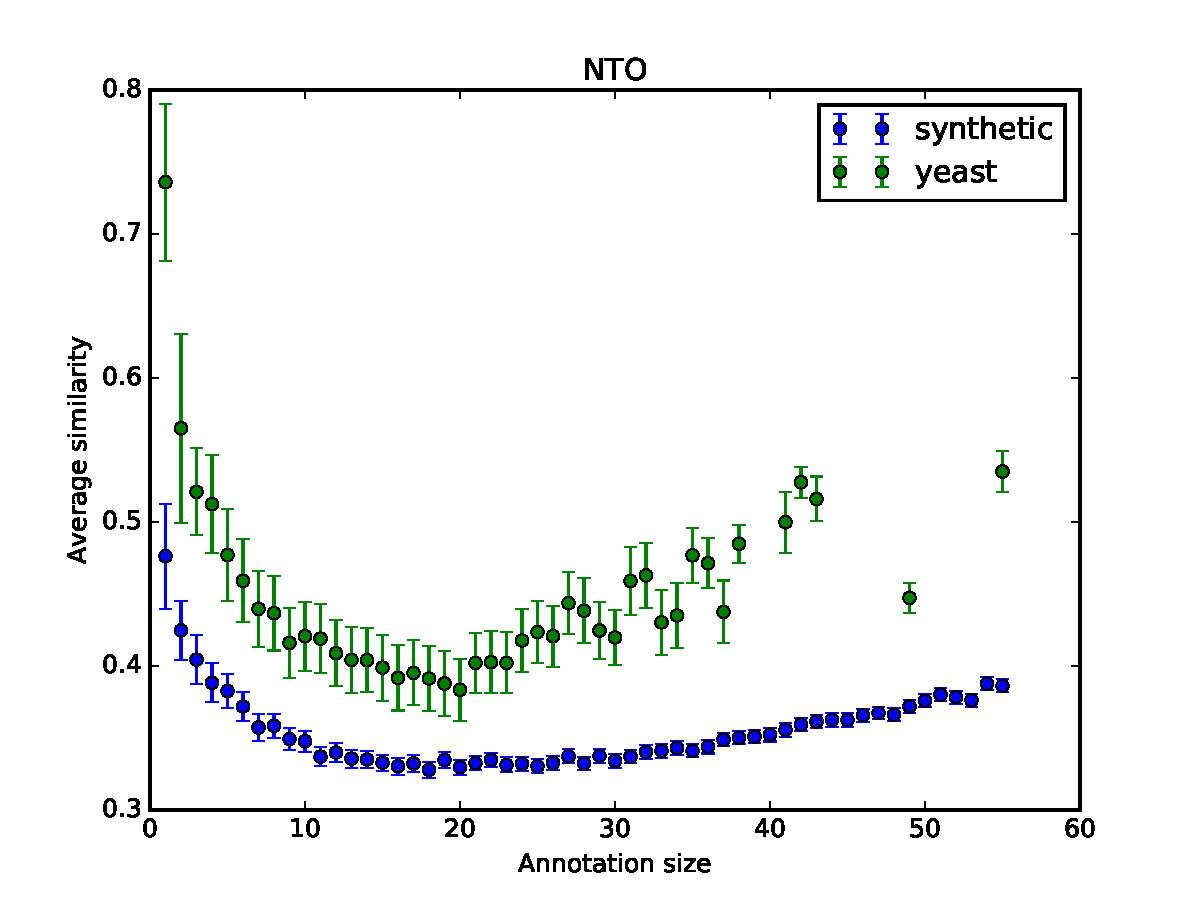
\includegraphics[width=0.5\linewidth, height=0.4\textheight]{groupwise/SIM_GROUPWISE_DAG_NTO_avg.pdf}
\end{figure}

\end{frame}

%------------------------------------------------

\begin{frame}{Pairwise Similarity Measures}

\begin{figure}
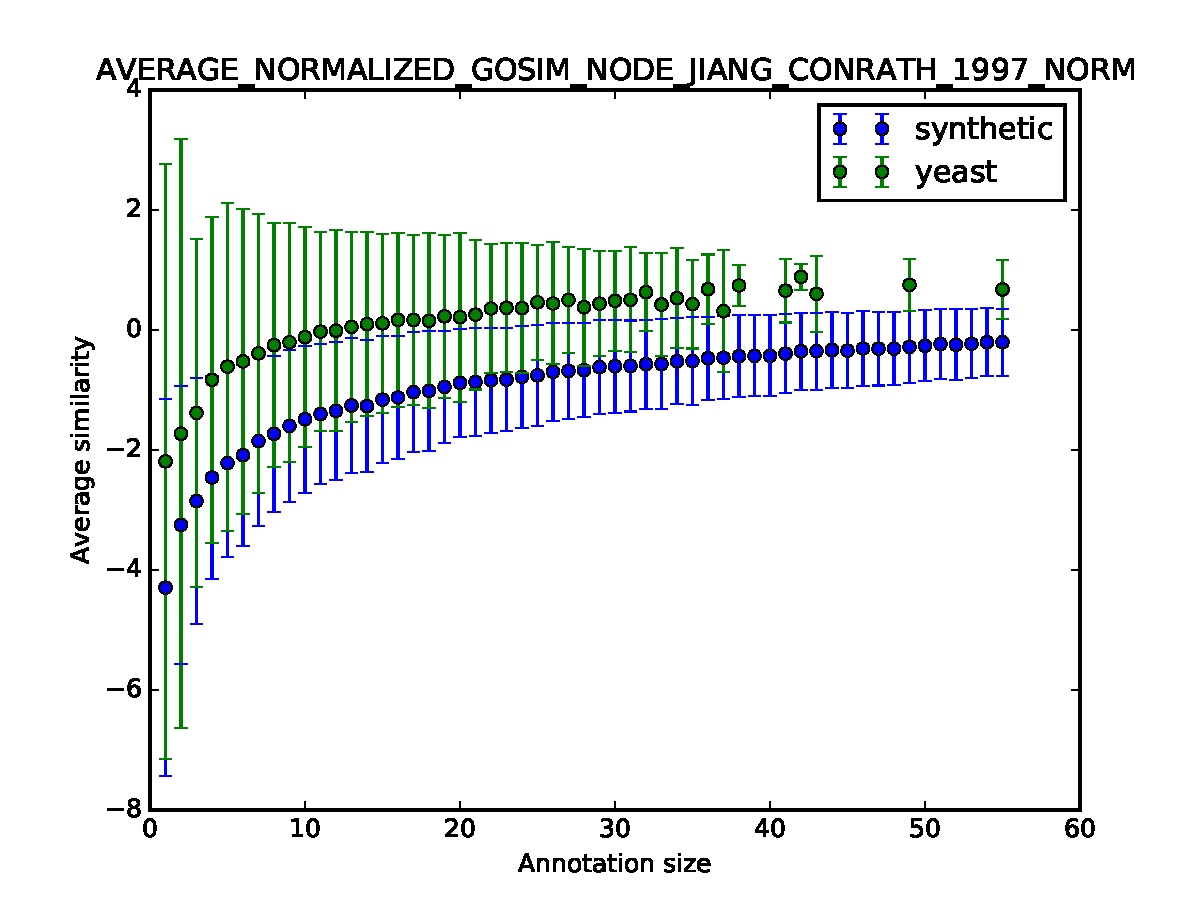
\includegraphics[width=0.5\linewidth, height=0.4\textheight]{pairwise/SIM_GROUPWISE_AVERAGE_NORMALIZED_GOSIM_SIM_PAIRWISE_DAG_NODE_JIANG_CONRATH_1997_NORM_avg.pdf}
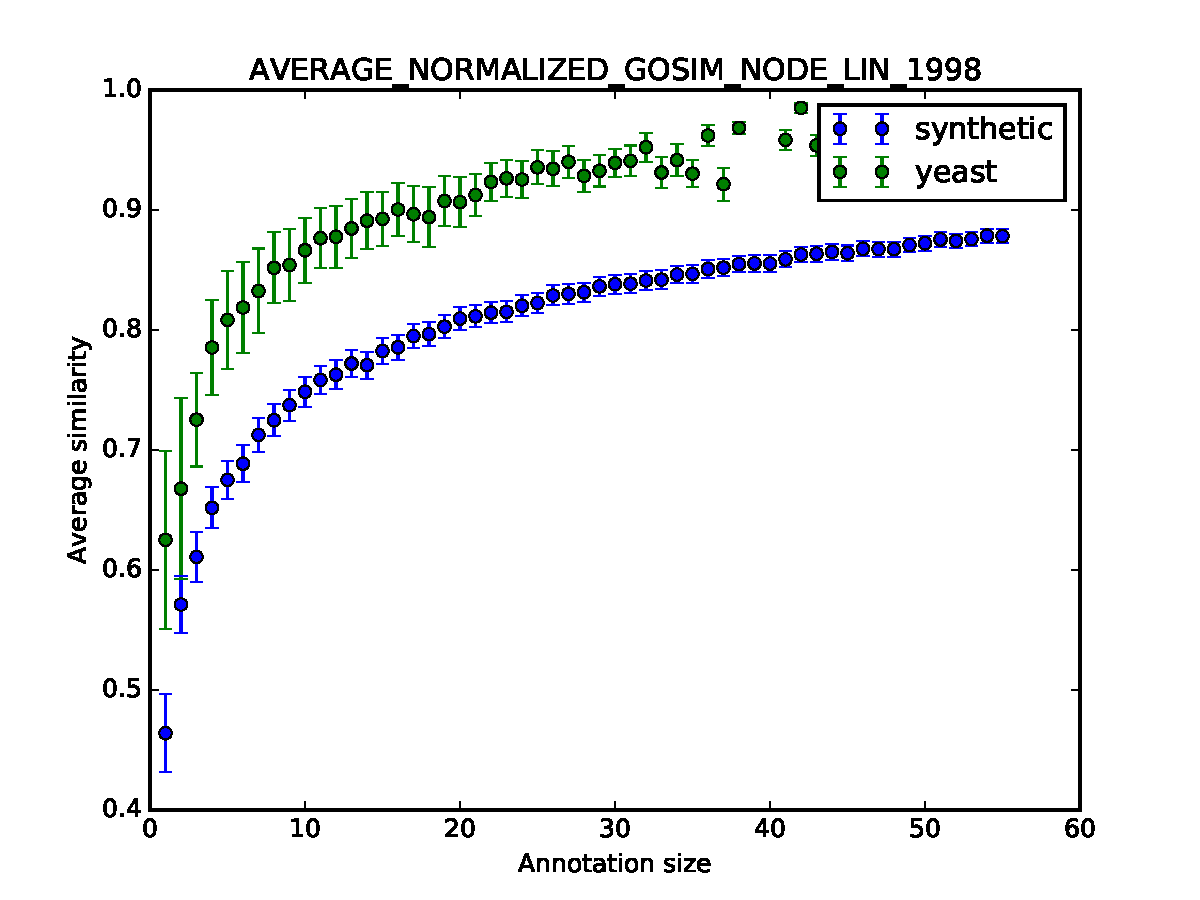
\includegraphics[width=0.5\linewidth, height=0.4\textheight]{pairwise/SIM_GROUPWISE_AVERAGE_NORMALIZED_GOSIM_SIM_PAIRWISE_DAG_NODE_LIN_1998_avg.pdf} \\
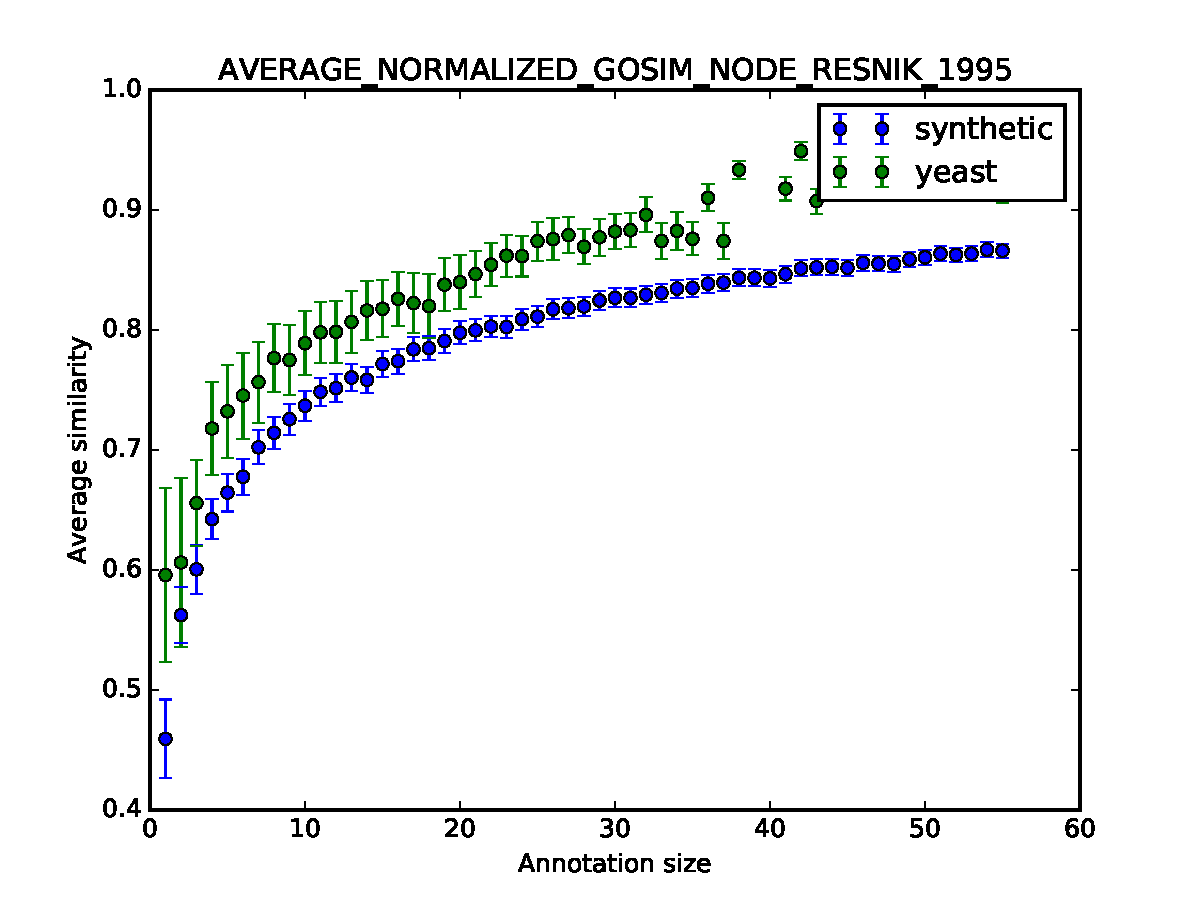
\includegraphics[width=0.5\linewidth, height=0.4\textheight]{pairwise/SIM_GROUPWISE_AVERAGE_NORMALIZED_GOSIM_SIM_PAIRWISE_DAG_NODE_RESNIK_1995_avg.pdf}
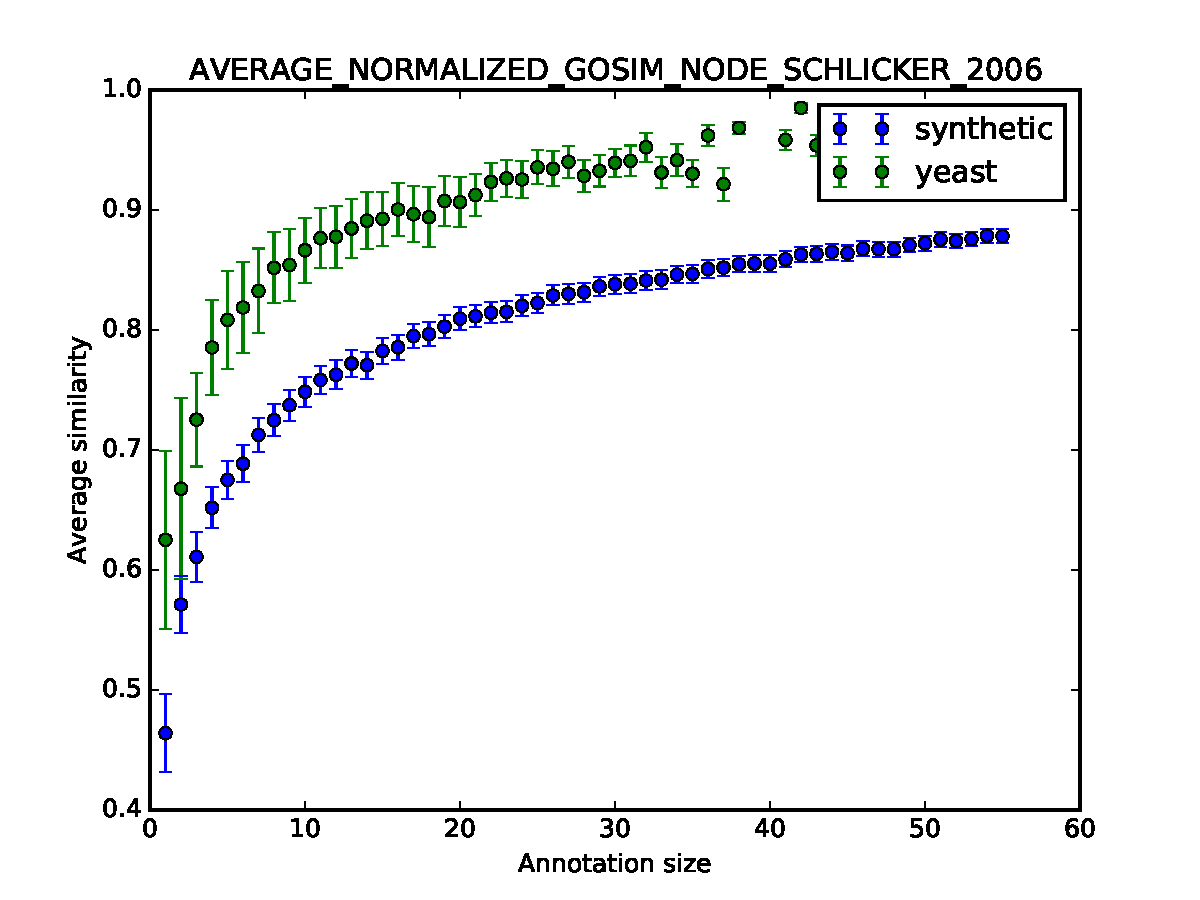
\includegraphics[width=0.5\linewidth, height=0.4\textheight]{pairwise/SIM_GROUPWISE_AVERAGE_NORMALIZED_GOSIM_SIM_PAIRWISE_DAG_NODE_SCHLICKER_2006_avg.pdf}
\end{figure}

\end{frame}


\begin{frame}{Pairwise Similarity Measures}

\begin{figure}
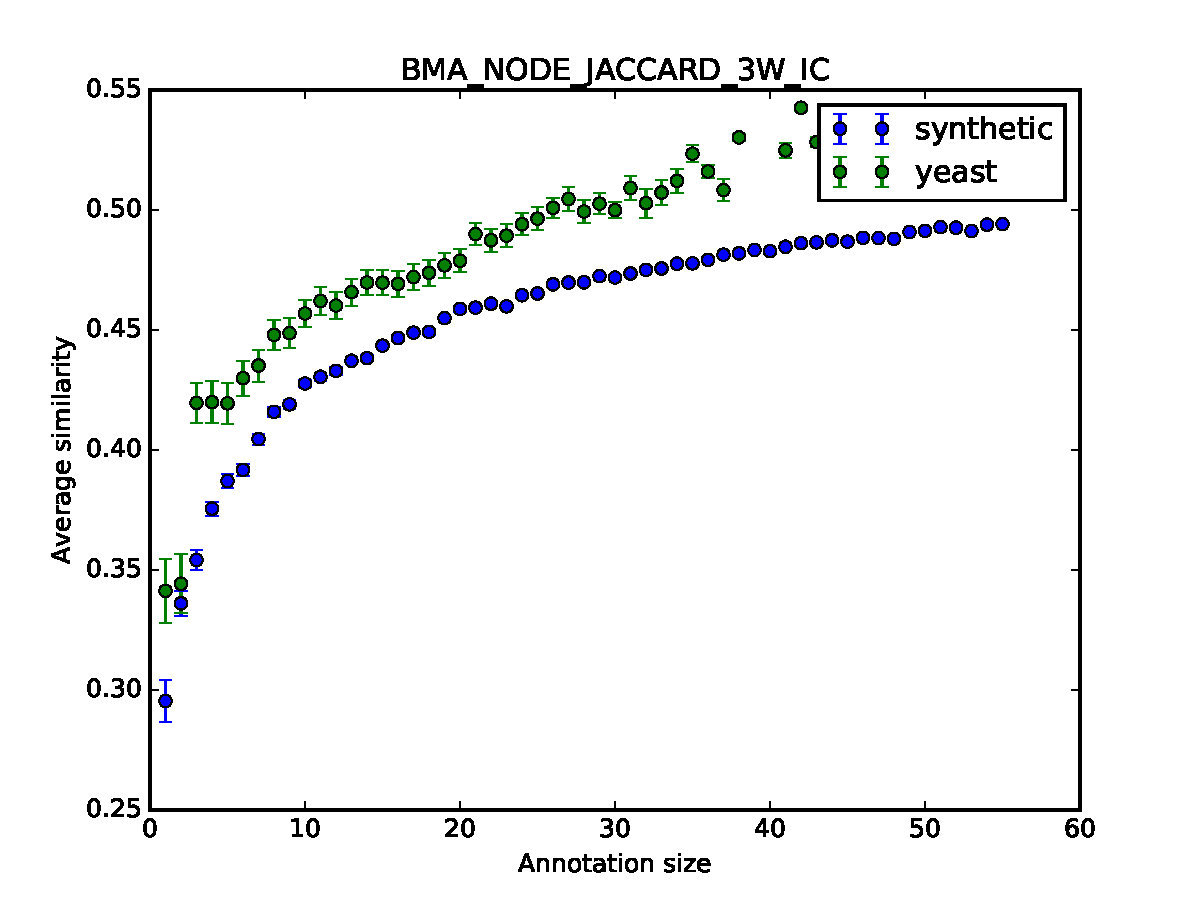
\includegraphics[width=0.5\linewidth, height=0.4\textheight]{pairwise/SIM_GROUPWISE_BMA_SIM_PAIRWISE_DAG_NODE_JACCARD_3W_IC_avg.pdf}
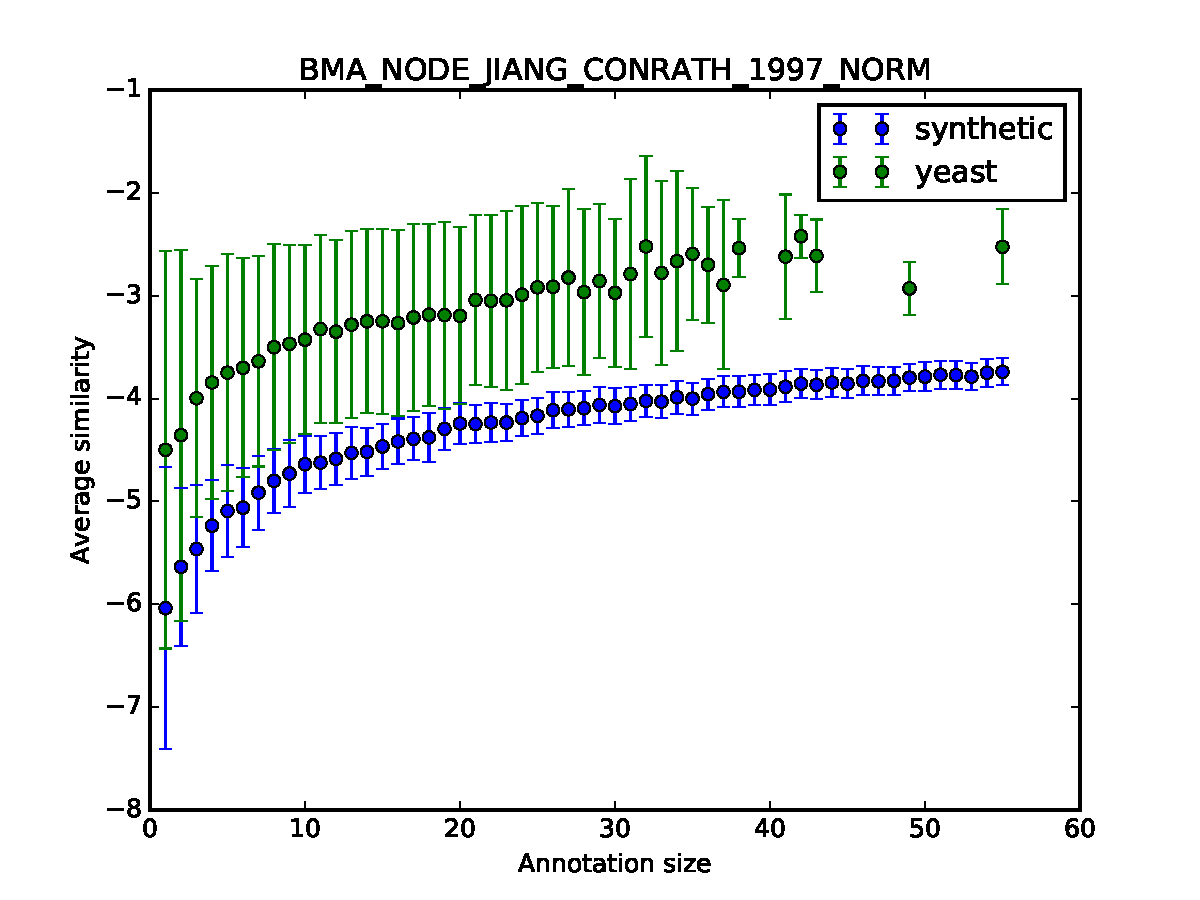
\includegraphics[width=0.5\linewidth, height=0.4\textheight]{pairwise/SIM_GROUPWISE_BMA_SIM_PAIRWISE_DAG_NODE_JIANG_CONRATH_1997_NORM_avg.pdf} \\
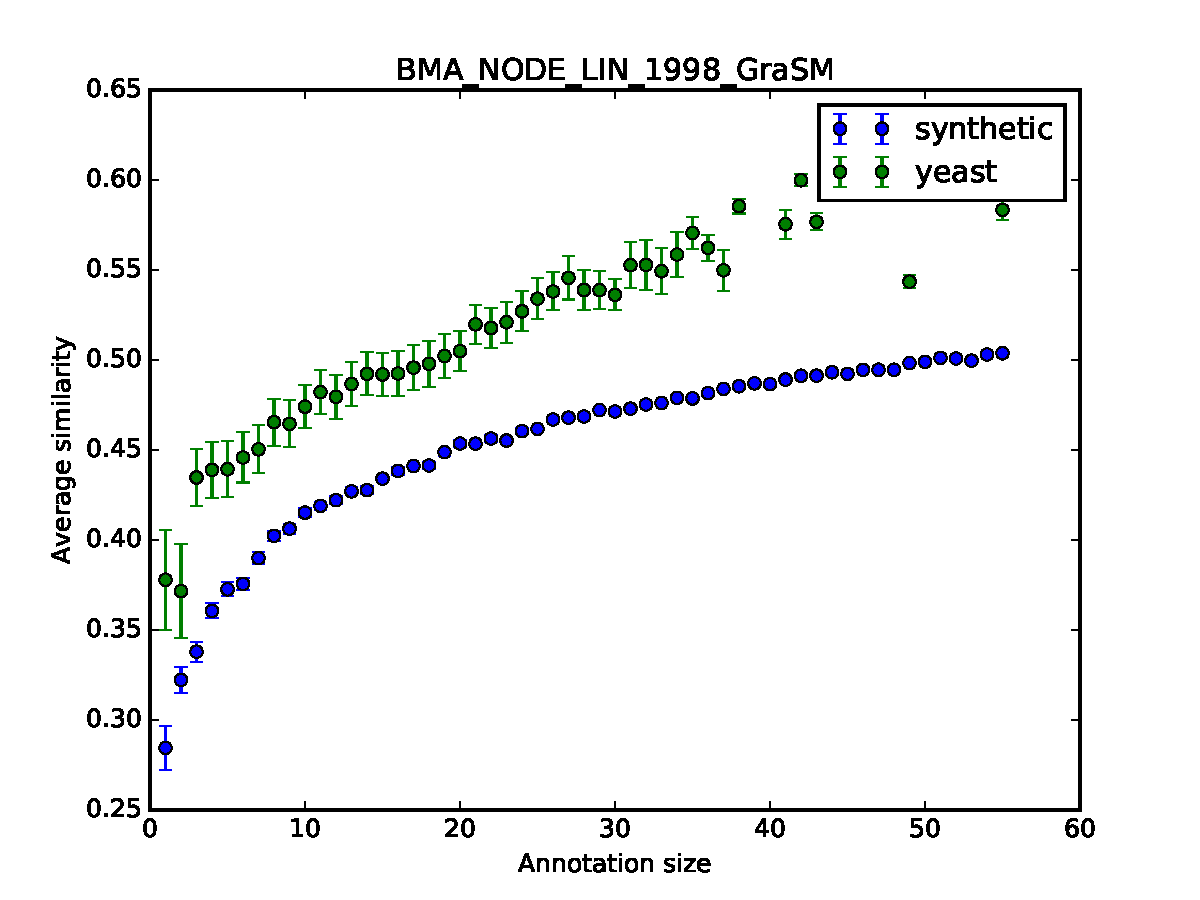
\includegraphics[width=0.5\linewidth, height=0.4\textheight]{pairwise/SIM_GROUPWISE_BMA_SIM_PAIRWISE_DAG_NODE_LIN_1998_GraSM_avg.pdf}
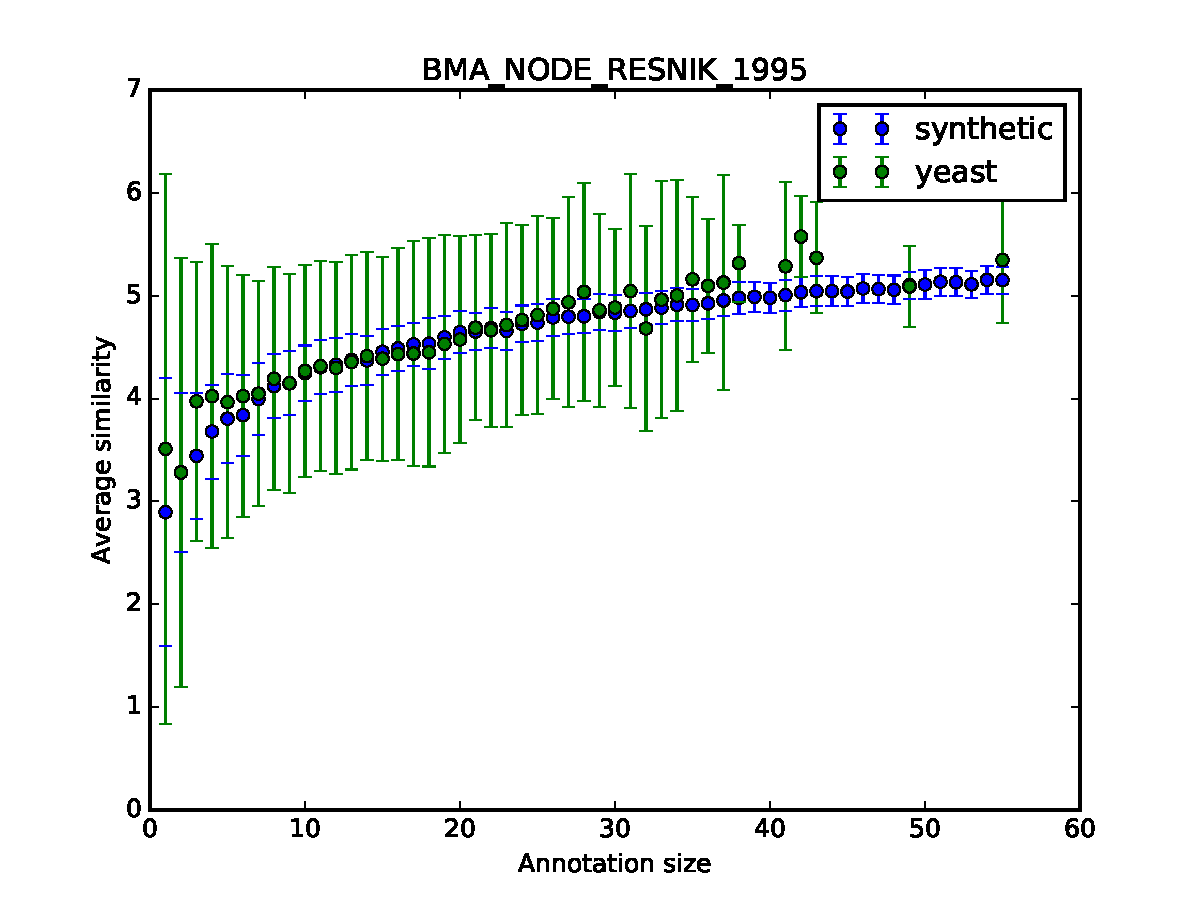
\includegraphics[width=0.5\linewidth, height=0.4\textheight]{pairwise/SIM_GROUPWISE_BMA_SIM_PAIRWISE_DAG_NODE_RESNIK_1995_avg.pdf}
\end{figure}

\end{frame}

\begin{frame}{Pairwise Similarity Measures}

\begin{figure}
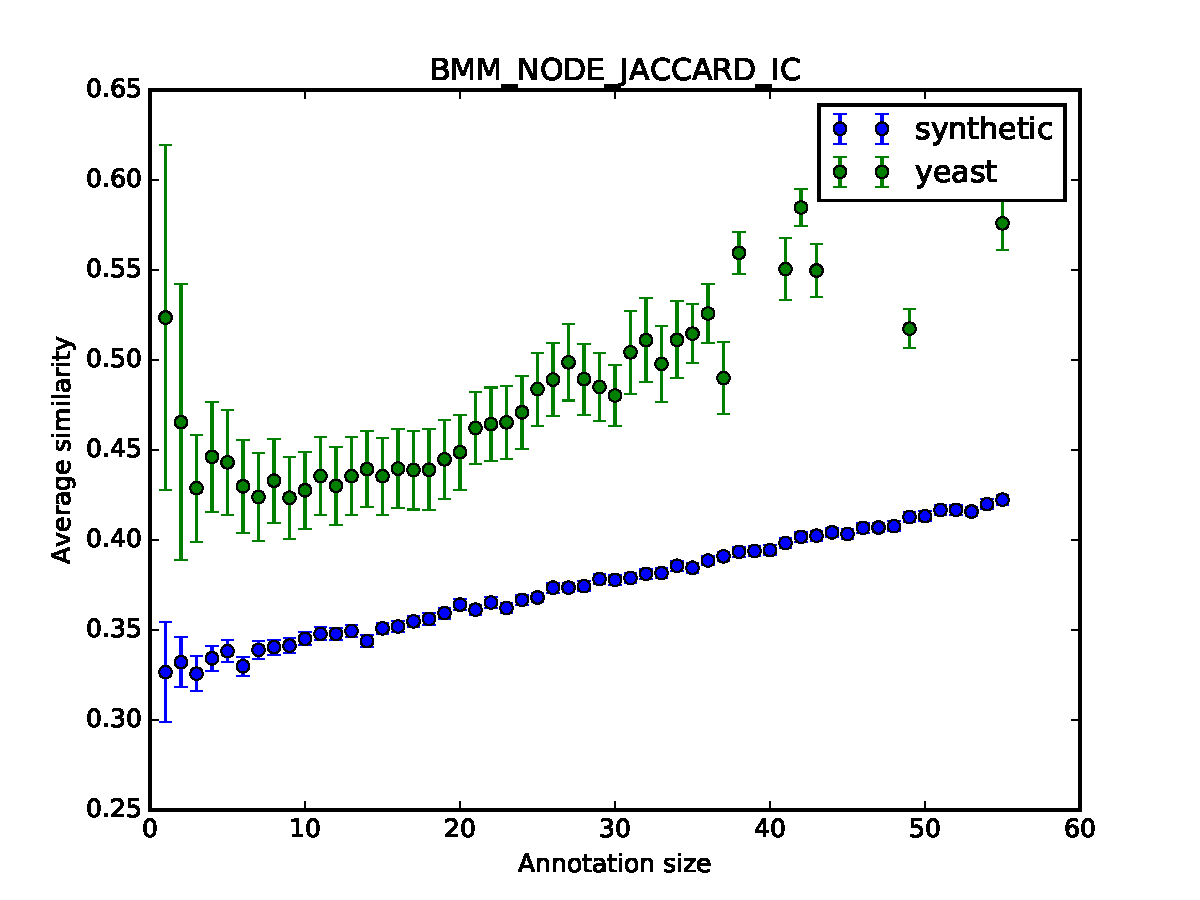
\includegraphics[width=0.5\linewidth, height=0.4\textheight]{pairwise/SIM_GROUPWISE_BMM_SIM_PAIRWISE_DAG_NODE_JACCARD_IC_avg.pdf}
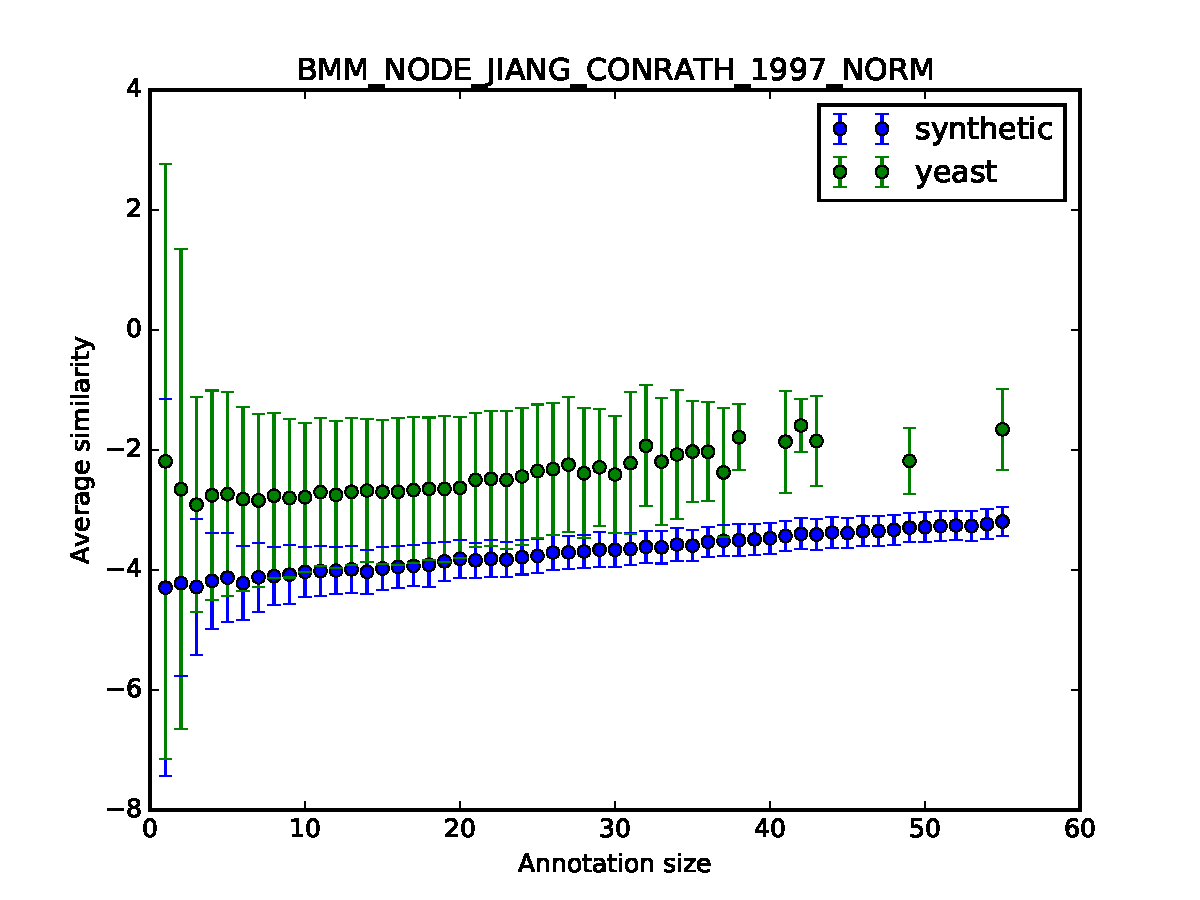
\includegraphics[width=0.5\linewidth, height=0.4\textheight]{pairwise/SIM_GROUPWISE_BMM_SIM_PAIRWISE_DAG_NODE_JIANG_CONRATH_1997_NORM_avg.pdf} \\
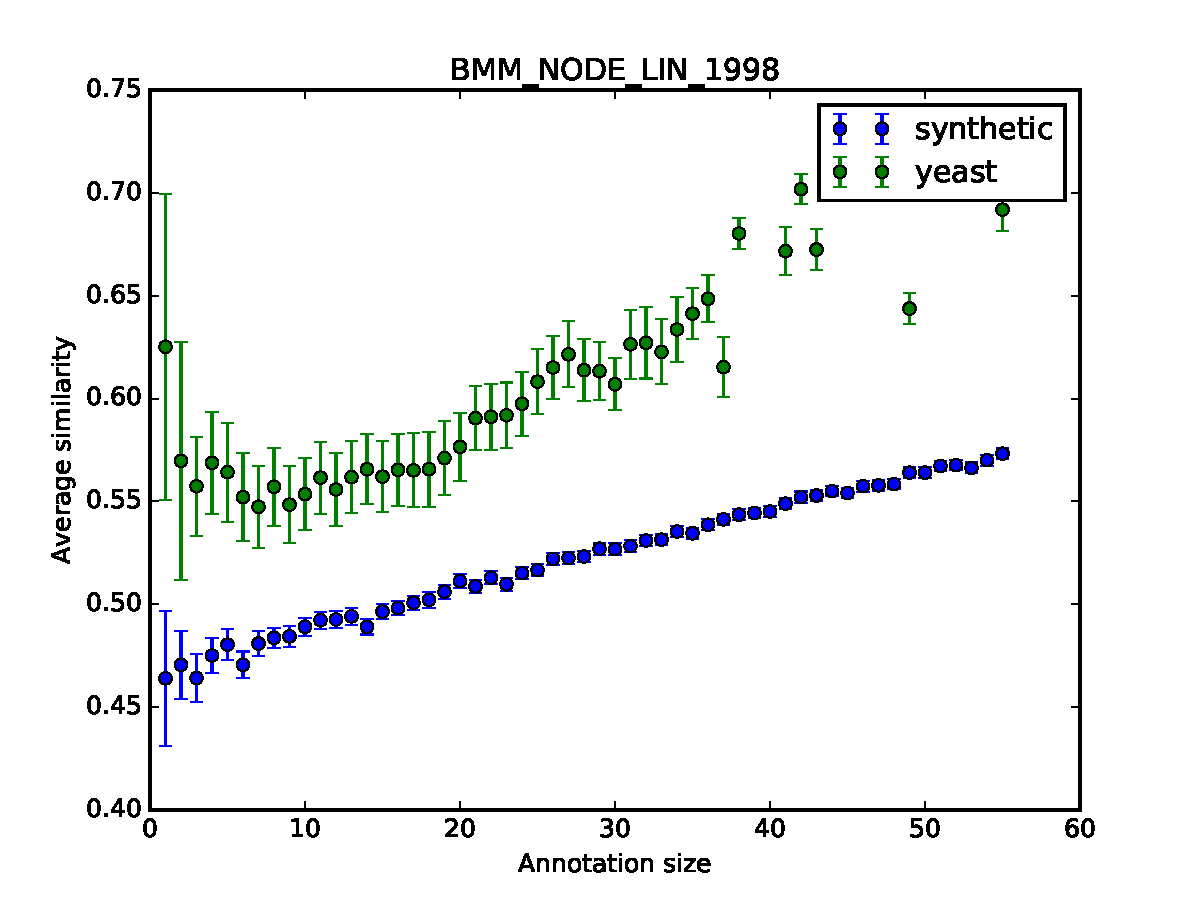
\includegraphics[width=0.5\linewidth, height=0.4\textheight]{pairwise/SIM_GROUPWISE_BMM_SIM_PAIRWISE_DAG_NODE_LIN_1998_avg.pdf}
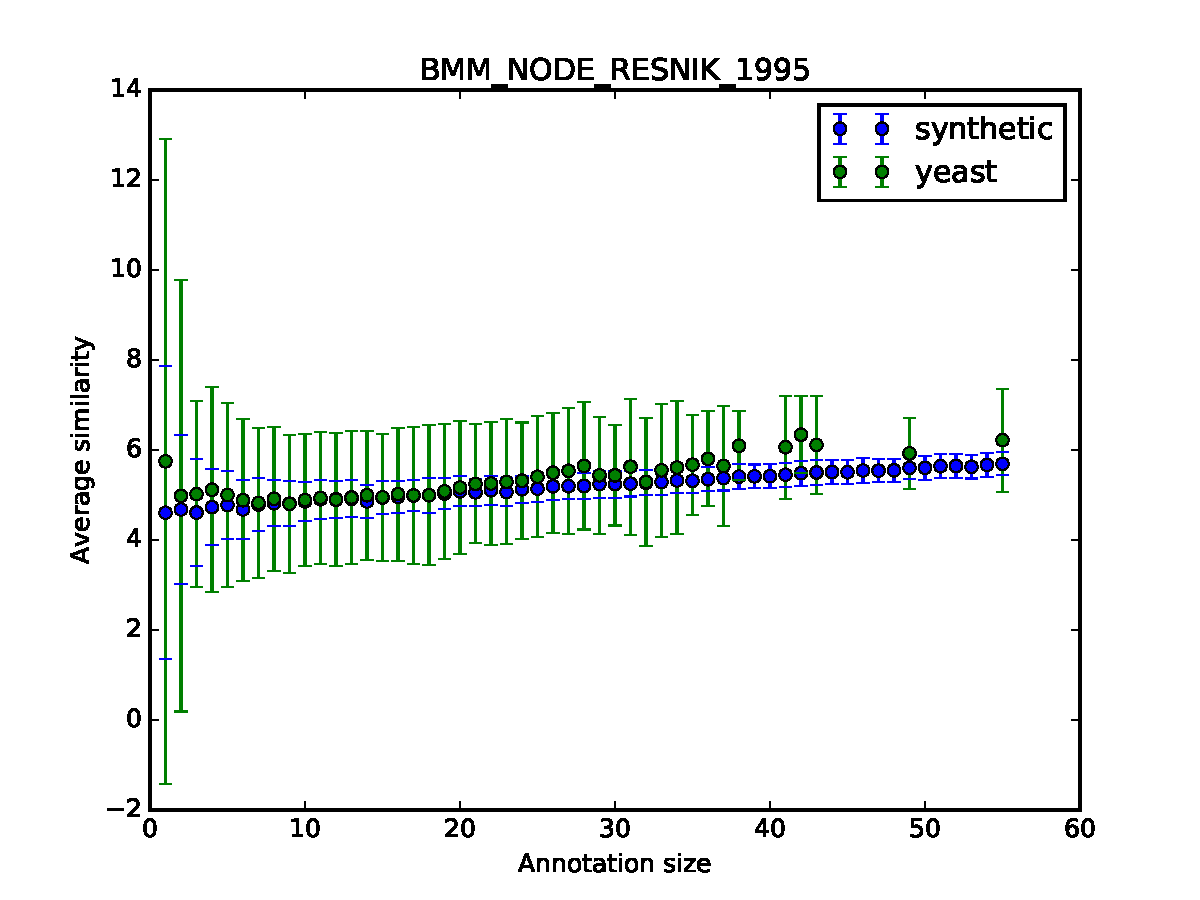
\includegraphics[width=0.5\linewidth, height=0.4\textheight]{pairwise/SIM_GROUPWISE_BMM_SIM_PAIRWISE_DAG_NODE_RESNIK_1995_avg.pdf}
\end{figure}

\end{frame}

\begin{frame}{Pairwise Similarity Measures}
\begin{figure}
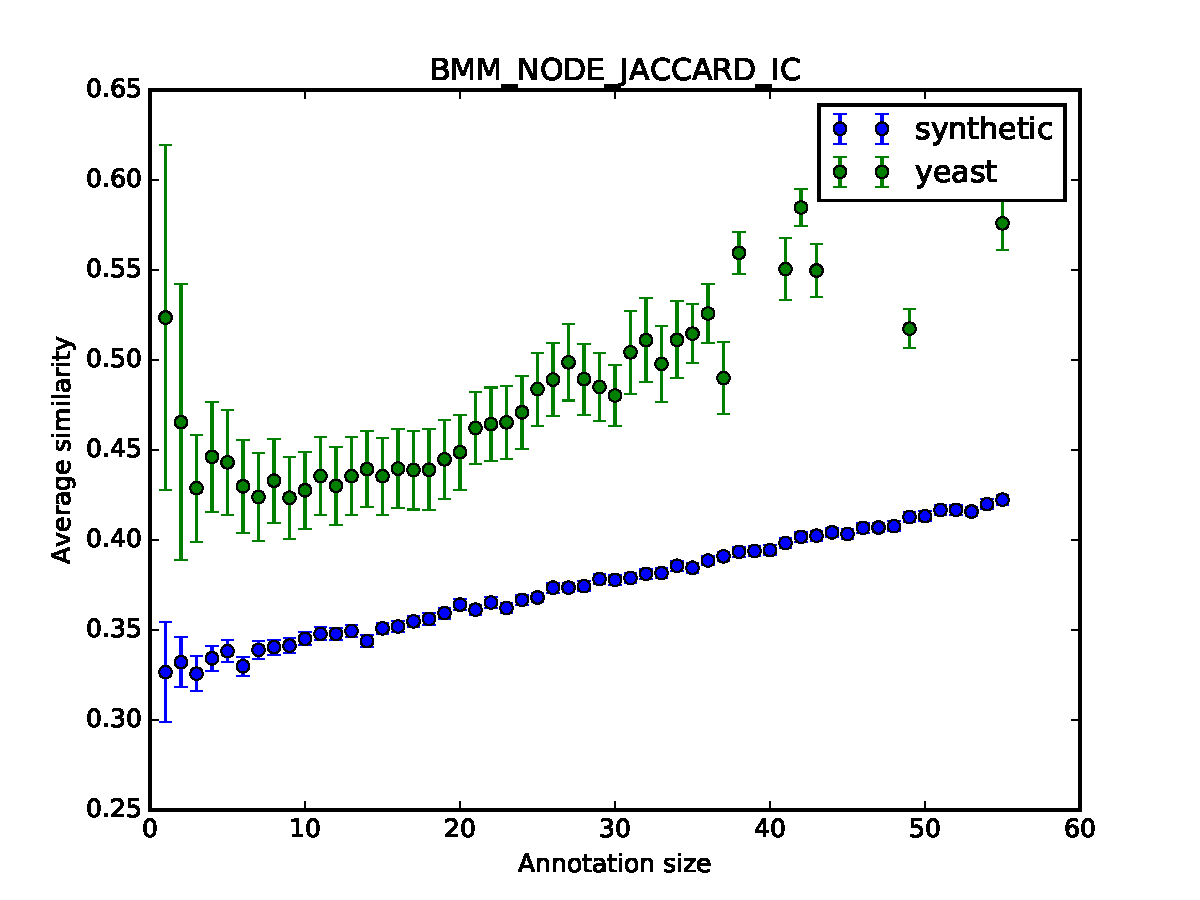
\includegraphics[width=0.5\linewidth, height=0.4\textheight]{pairwise/SIM_GROUPWISE_BMM_SIM_PAIRWISE_DAG_NODE_JACCARD_IC_avg.pdf}
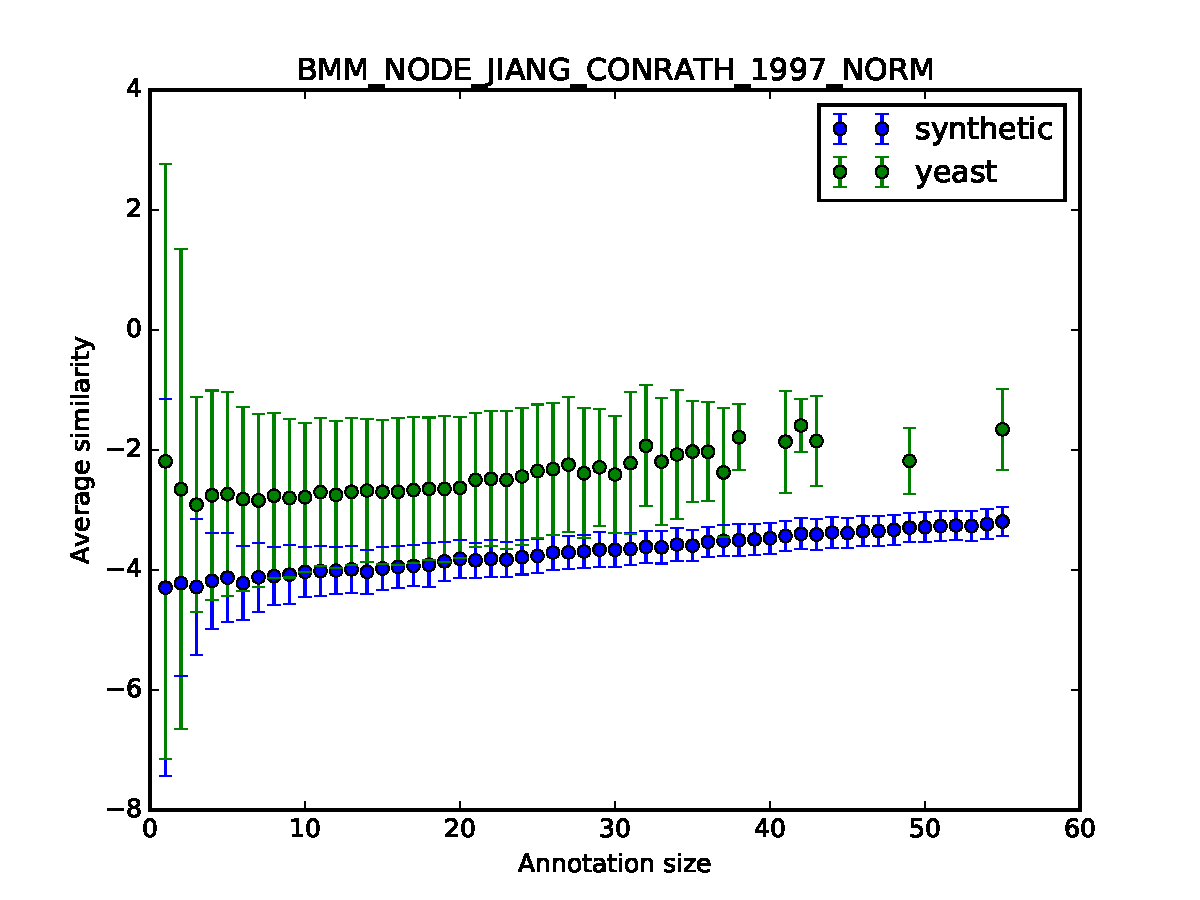
\includegraphics[width=0.5\linewidth, height=0.4\textheight]{pairwise/SIM_GROUPWISE_BMM_SIM_PAIRWISE_DAG_NODE_JIANG_CONRATH_1997_NORM_avg.pdf} \\
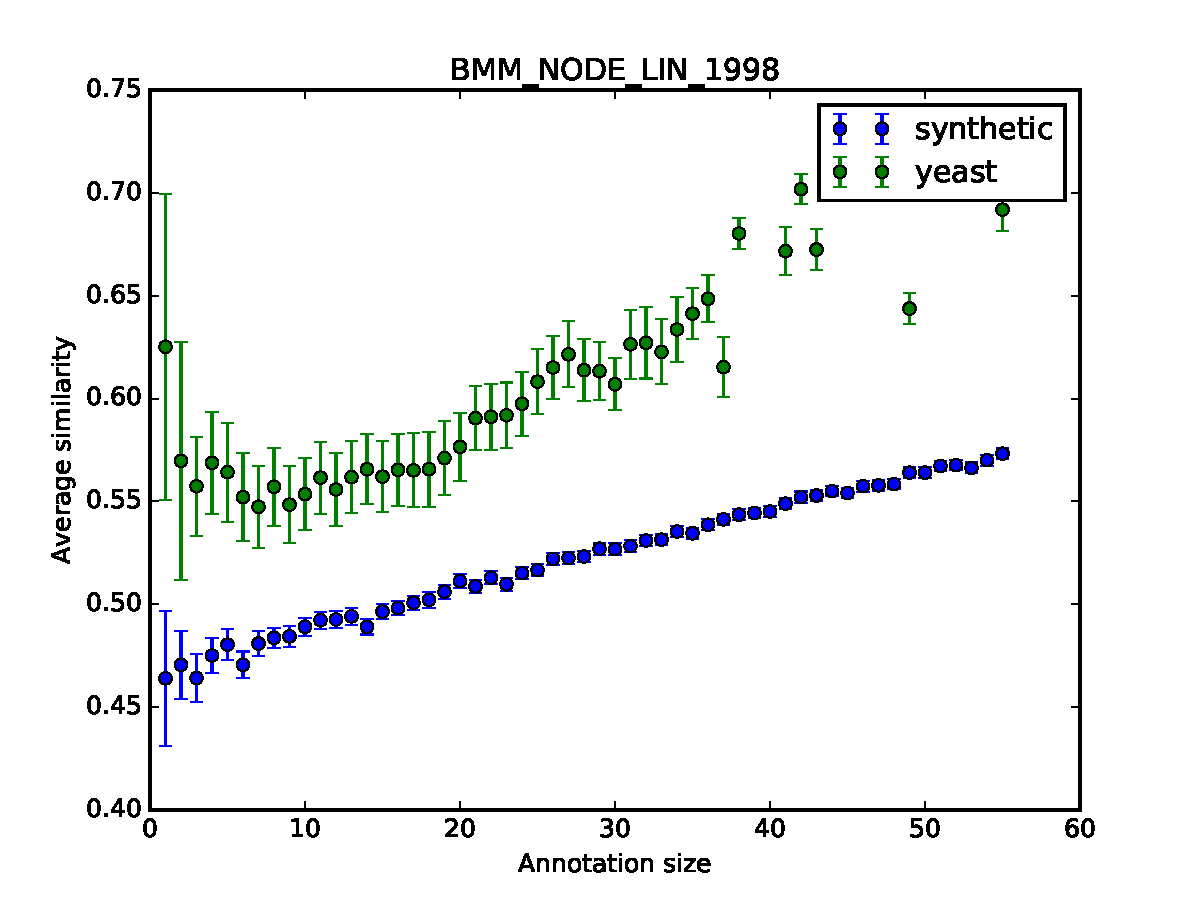
\includegraphics[width=0.5\linewidth, height=0.4\textheight]{pairwise/SIM_GROUPWISE_BMM_SIM_PAIRWISE_DAG_NODE_LIN_1998_avg.pdf}
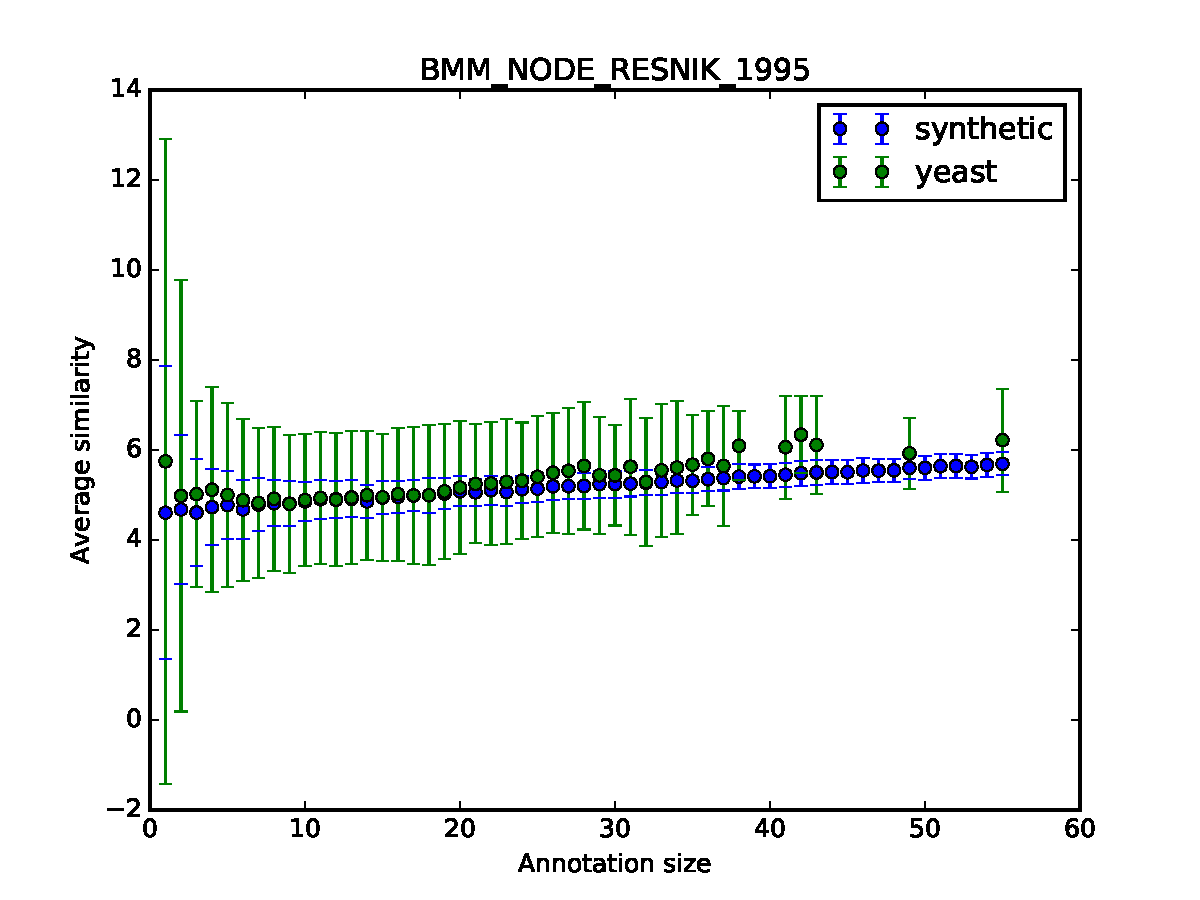
\includegraphics[width=0.5\linewidth, height=0.4\textheight]{pairwise/SIM_GROUPWISE_BMM_SIM_PAIRWISE_DAG_NODE_RESNIK_1995_avg.pdf}
\end{figure}
\end{frame}

\begin{frame}{Pairwise Similarity Measures}
\begin{figure}
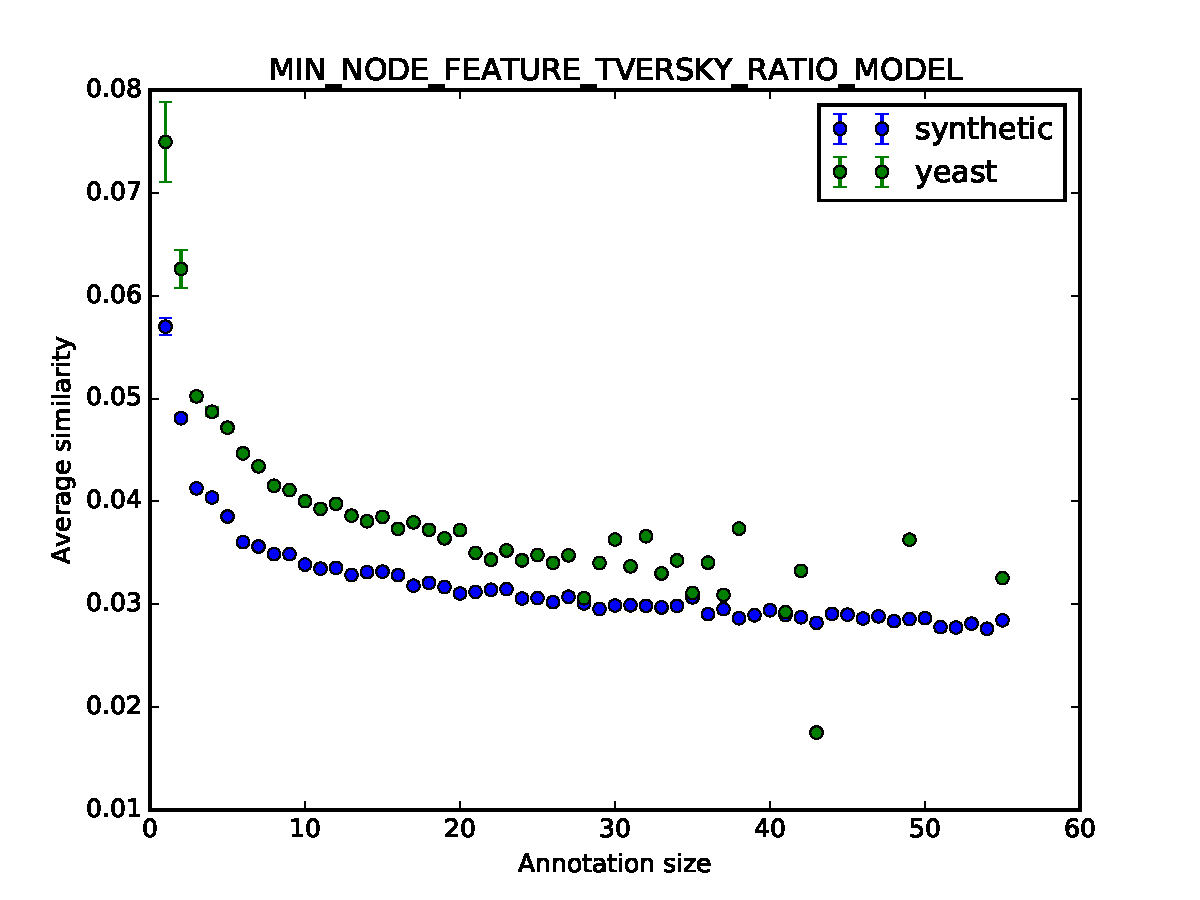
\includegraphics[width=0.5\linewidth, height=0.4\textheight]{pairwise/SIM_GROUPWISE_MIN_SIM_PAIRWISE_DAG_NODE_FEATURE_TVERSKY_RATIO_MODEL_avg.pdf}
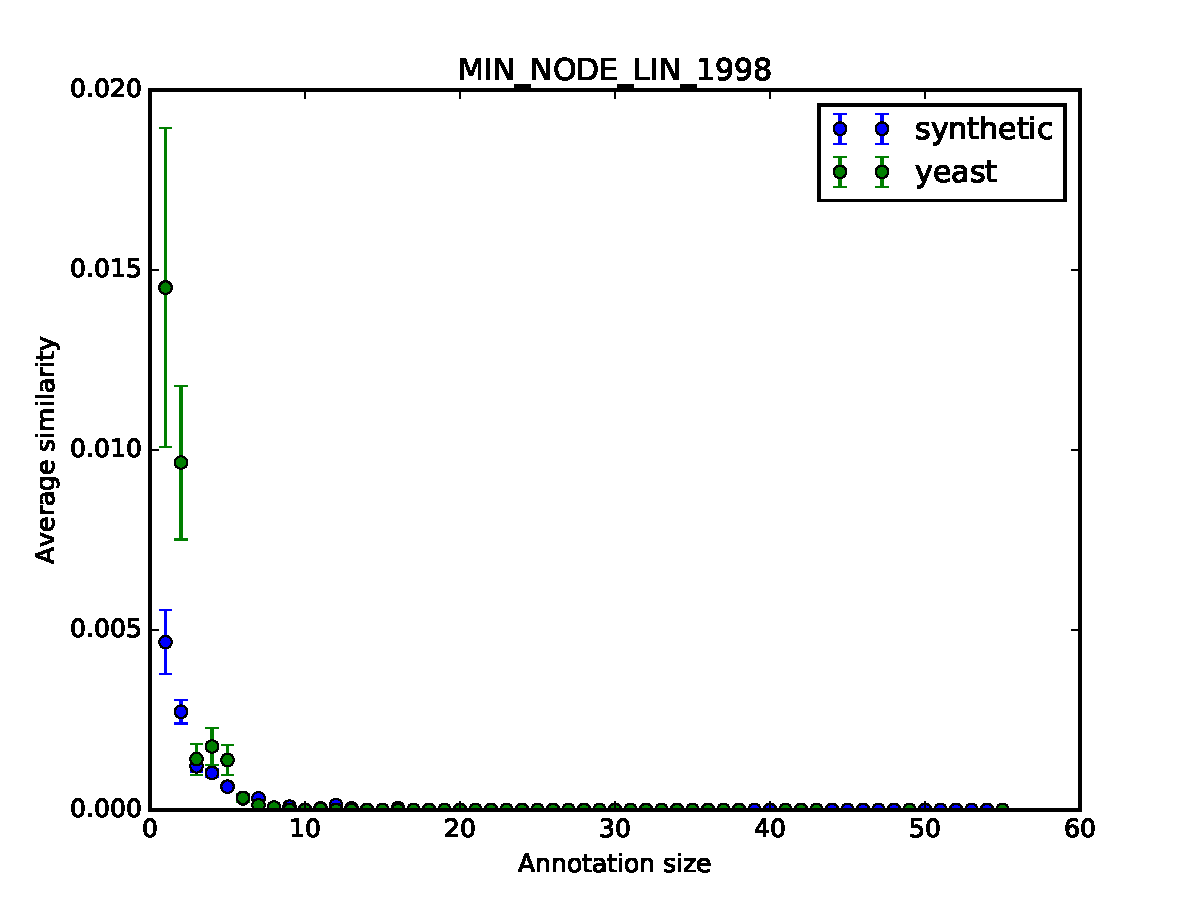
\includegraphics[width=0.5\linewidth, height=0.4\textheight]{pairwise/SIM_GROUPWISE_MIN_SIM_PAIRWISE_DAG_NODE_LIN_1998_avg.pdf} \\
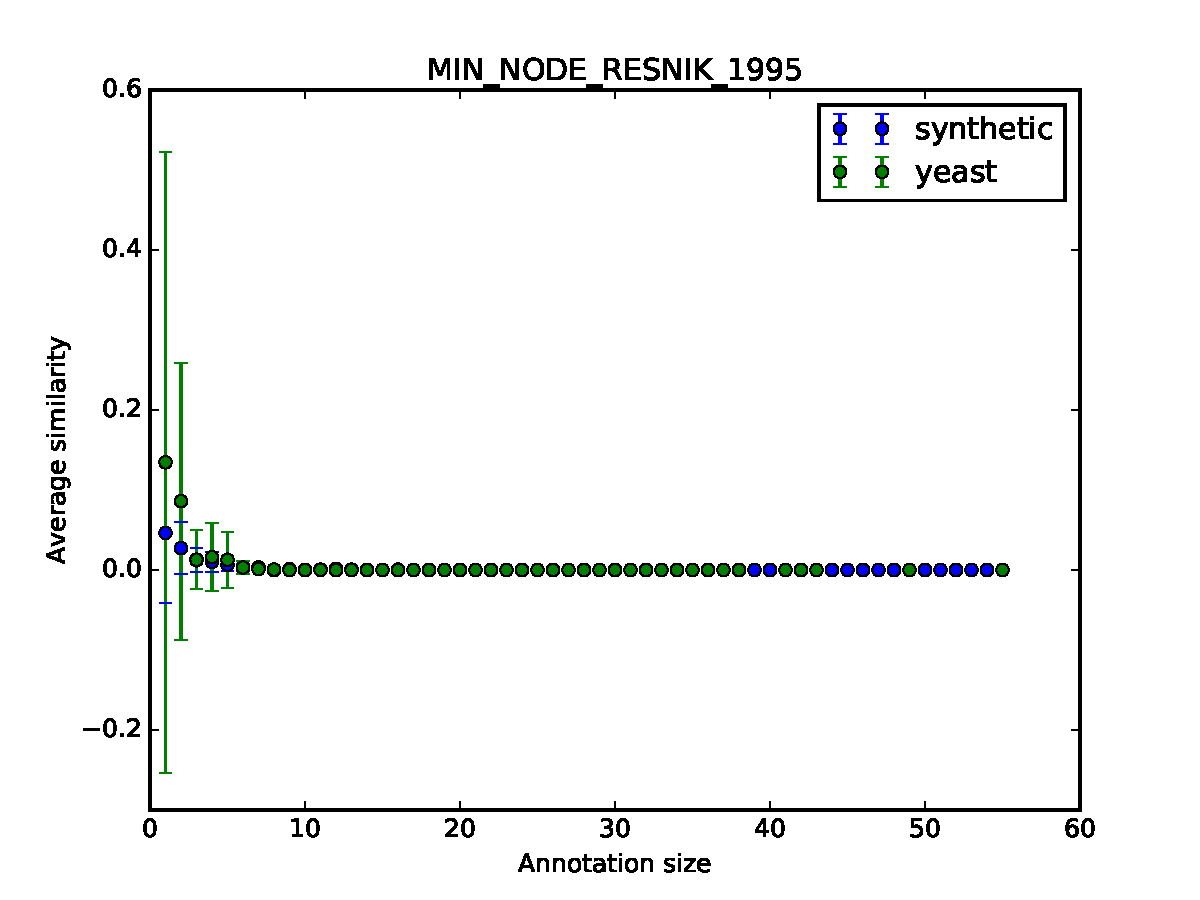
\includegraphics[width=0.5\linewidth, height=0.4\textheight]{pairwise/SIM_GROUPWISE_MIN_SIM_PAIRWISE_DAG_NODE_RESNIK_1995_avg.pdf}
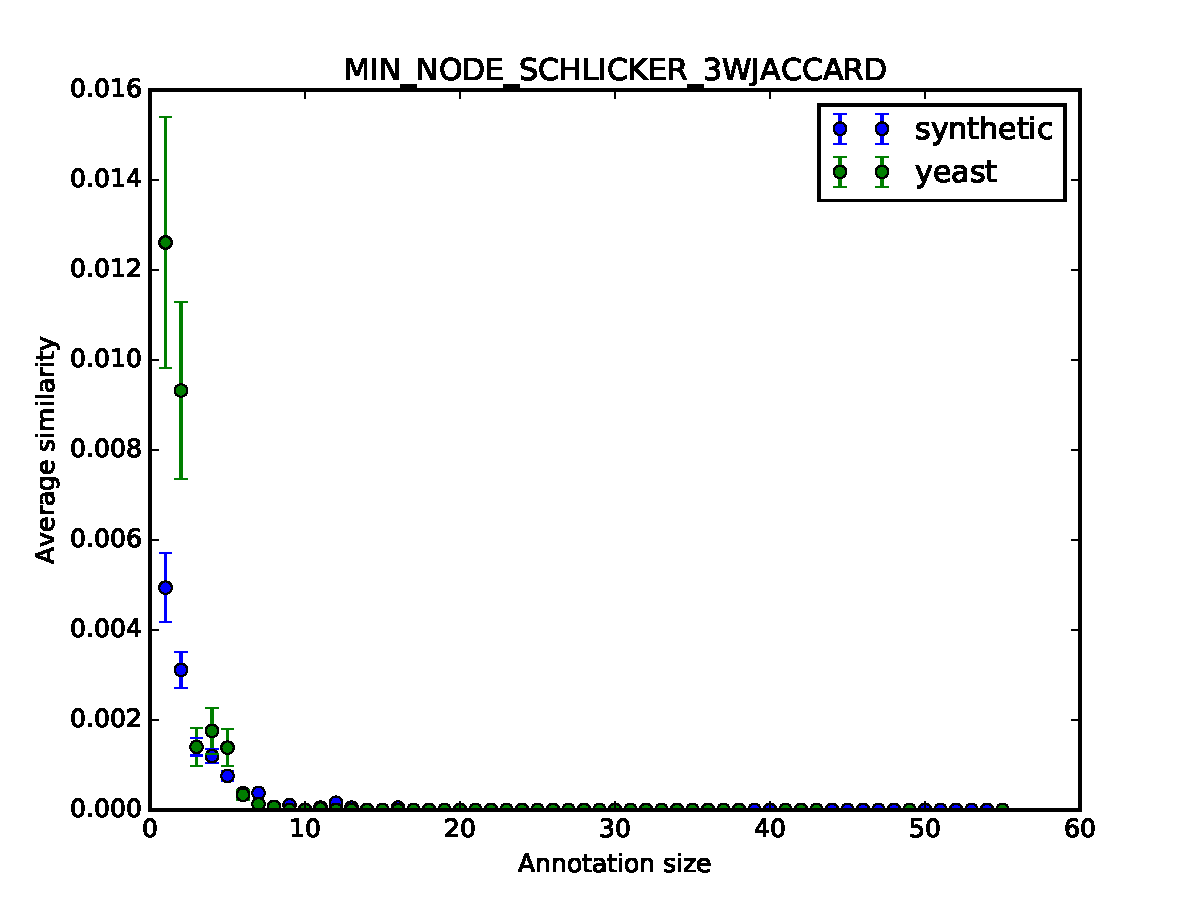
\includegraphics[width=0.5\linewidth, height=0.4\textheight]{pairwise/SIM_GROUPWISE_MIN_SIM_PAIRWISE_DAG_NODE_SCHLICKER_3WJACCARD_avg.pdf}
\end{figure}
\end{frame}


\begin{frame}{Pairwise Similarity Measures}
\begin{figure}
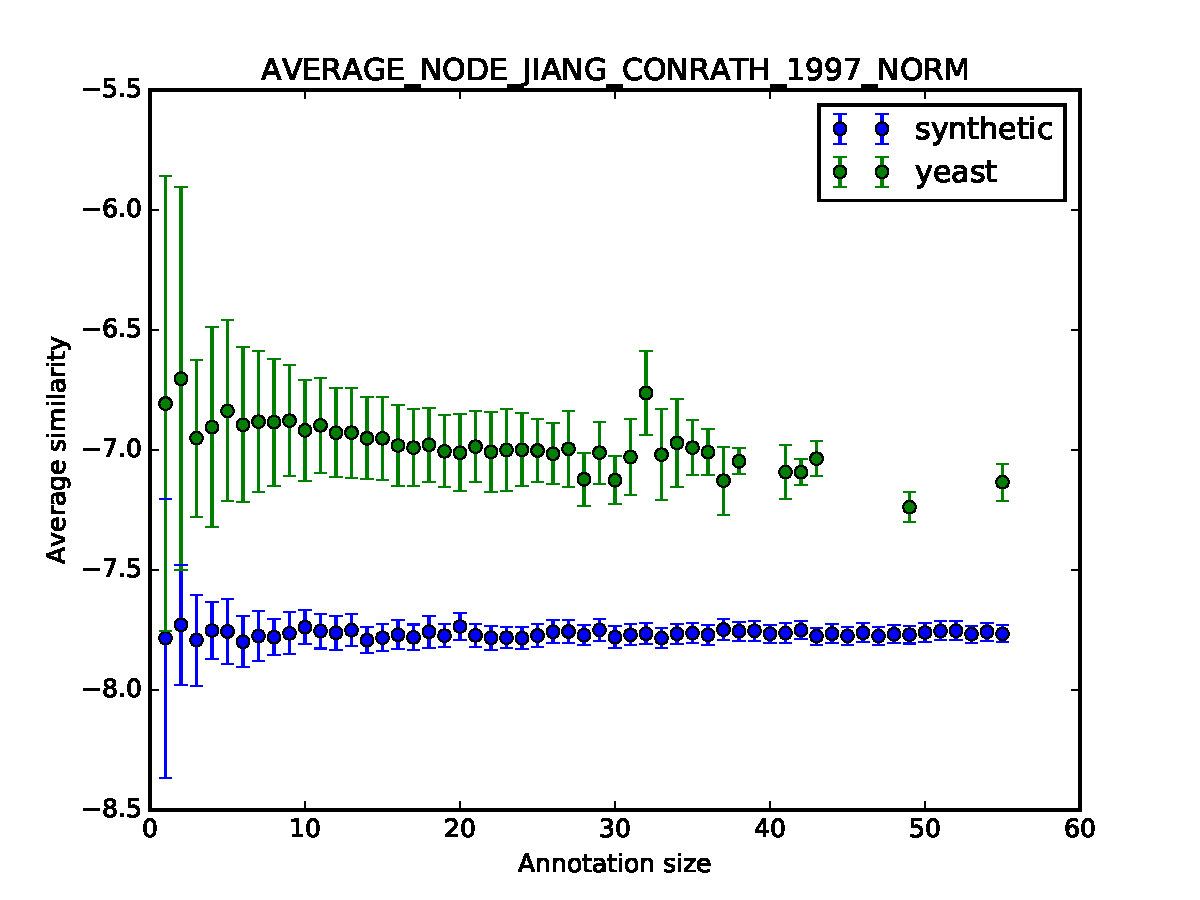
\includegraphics[width=0.5\linewidth, height=0.4\textheight]{pairwise/SIM_GROUPWISE_AVERAGE_SIM_PAIRWISE_DAG_NODE_JIANG_CONRATH_1997_NORM_avg.pdf}
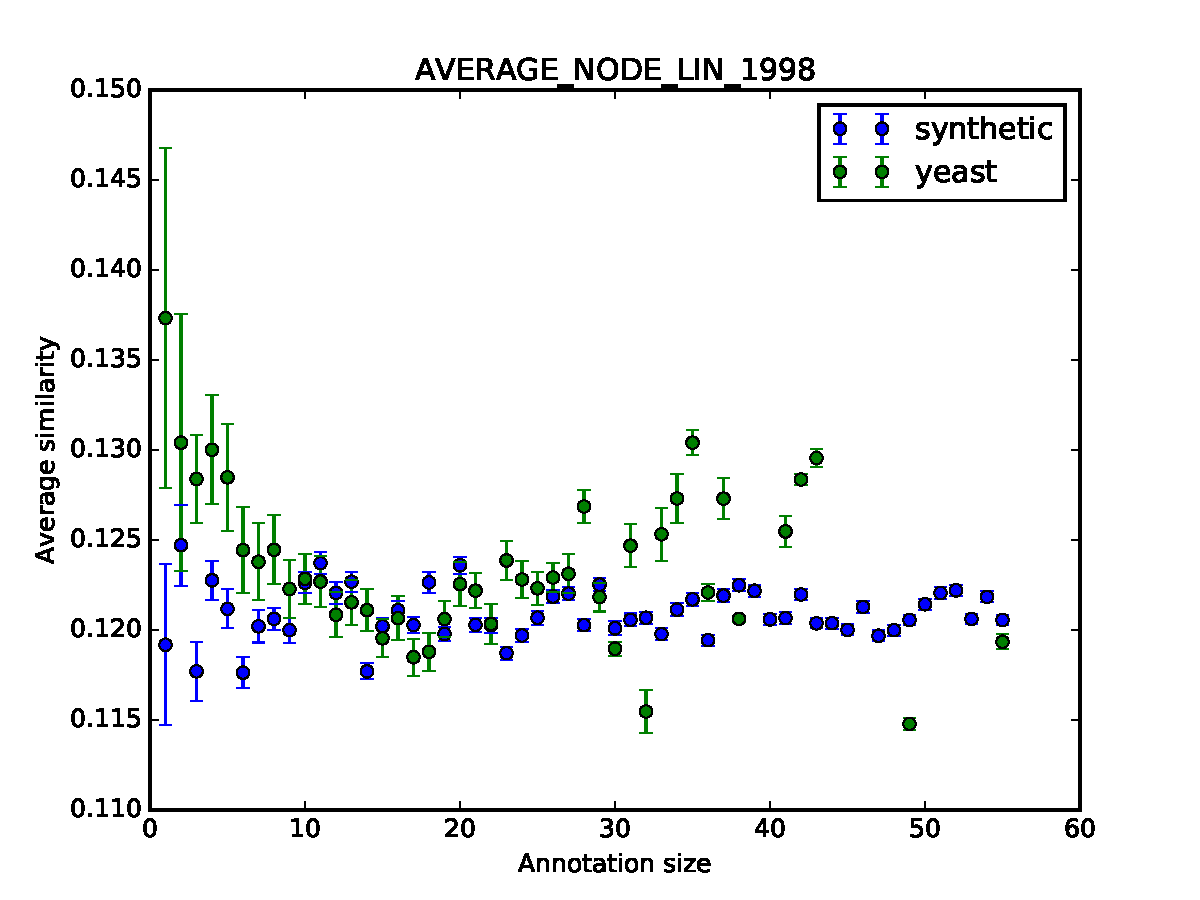
\includegraphics[width=0.5\linewidth, height=0.4\textheight]{pairwise/SIM_GROUPWISE_AVERAGE_SIM_PAIRWISE_DAG_NODE_LIN_1998_avg.pdf} \\
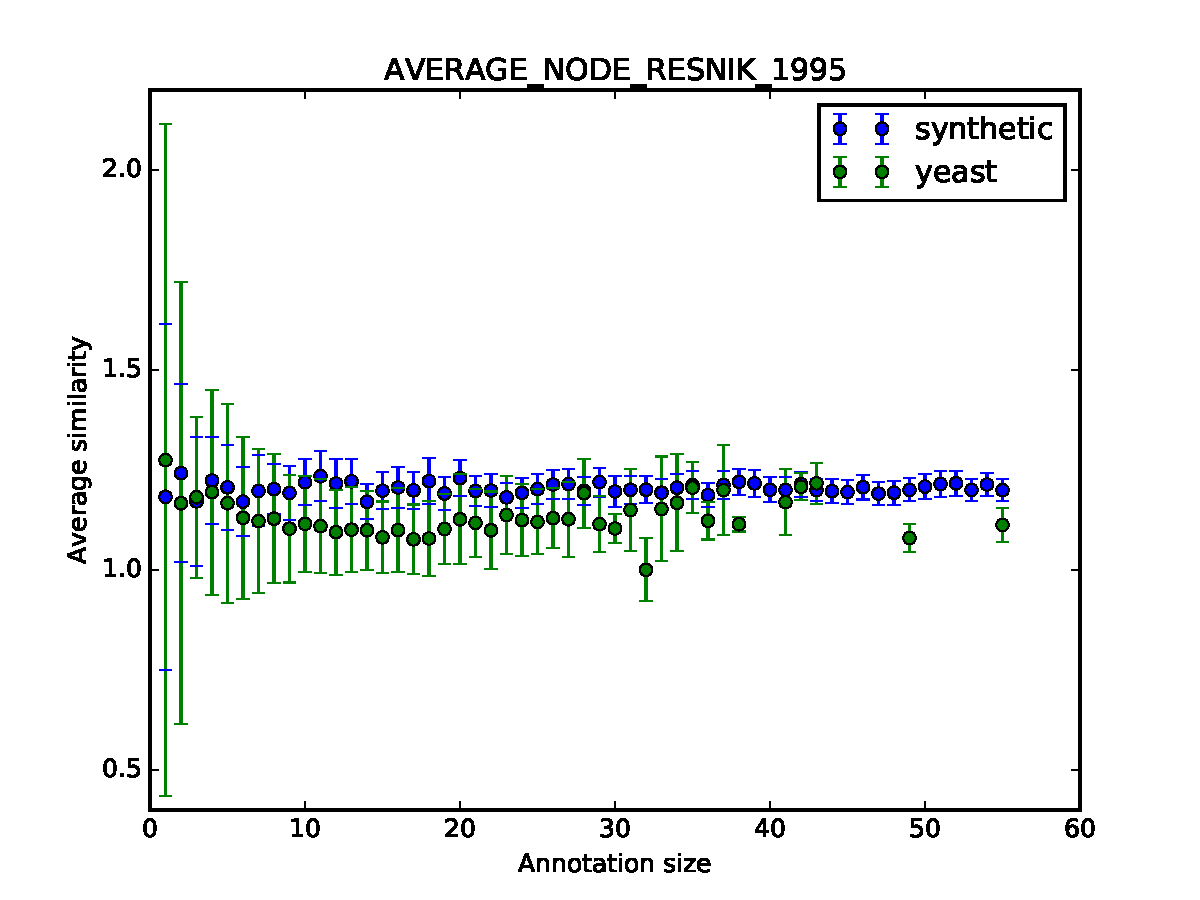
\includegraphics[width=0.5\linewidth, height=0.4\textheight]{pairwise/SIM_GROUPWISE_AVERAGE_SIM_PAIRWISE_DAG_NODE_RESNIK_1995_avg.pdf}
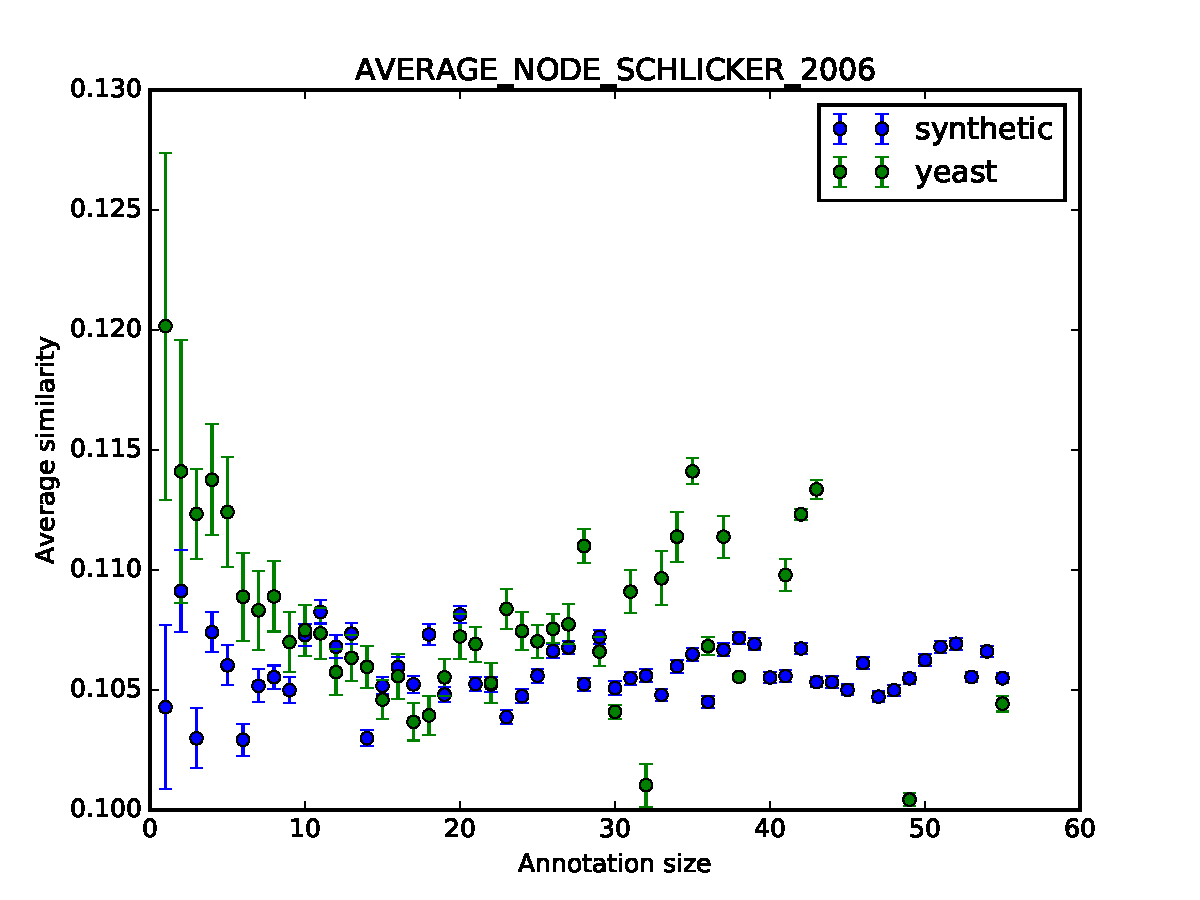
\includegraphics[width=0.5\linewidth, height=0.4\textheight]{pairwise/SIM_GROUPWISE_AVERAGE_SIM_PAIRWISE_DAG_NODE_SCHLICKER_2006_avg.pdf}
\end{figure}
\end{frame}


\begin{frame}{Pairwise Similarity Measures}
\begin{figure}
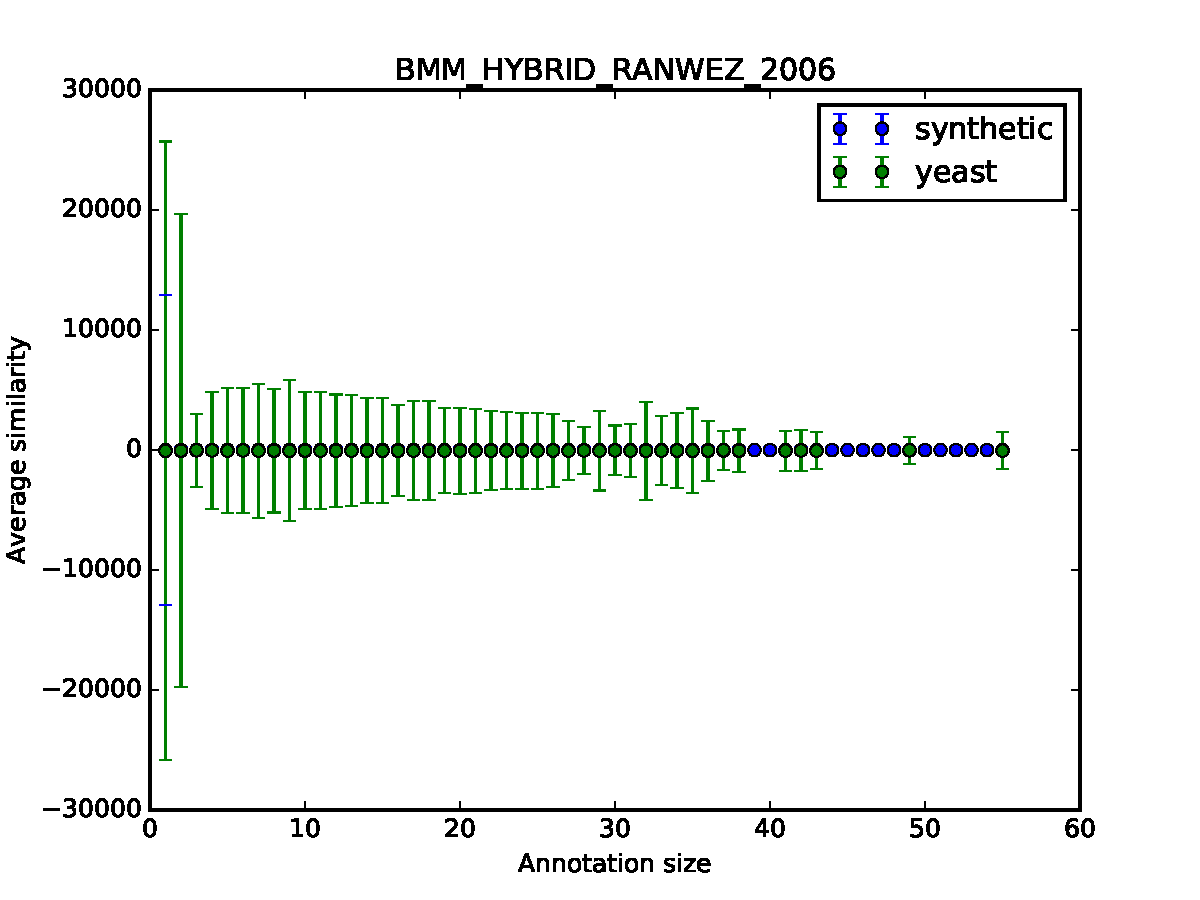
\includegraphics[width=0.5\linewidth, height=0.4\textheight]{pairwise/SIM_GROUPWISE_BMM_SIM_PAIRWISE_DAG_HYBRID_RANWEZ_2006_avg.pdf}
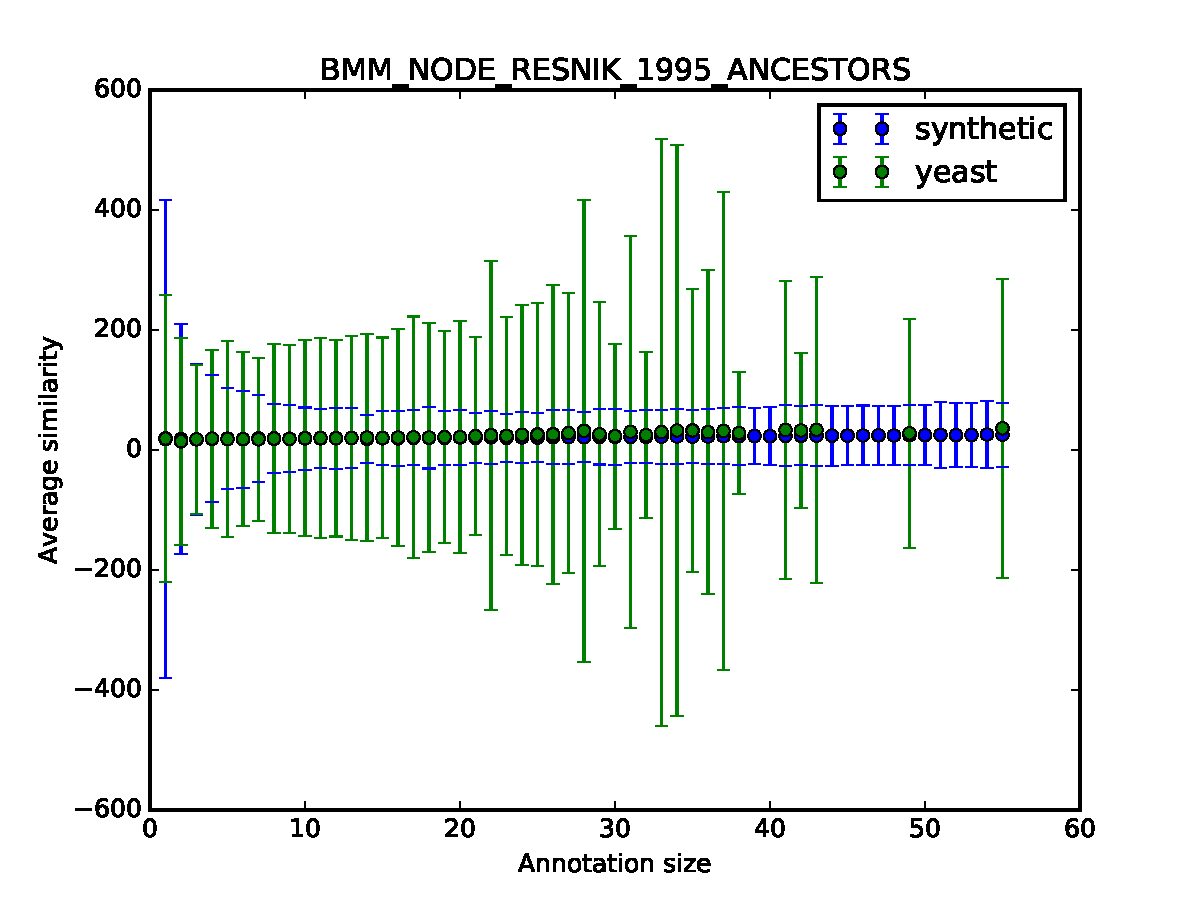
\includegraphics[width=0.5\linewidth, height=0.4\textheight]{pairwise/SIM_GROUPWISE_BMM_SIM_PAIRWISE_DAG_NODE_RESNIK_1995_ANCESTORS_avg.pdf} \\
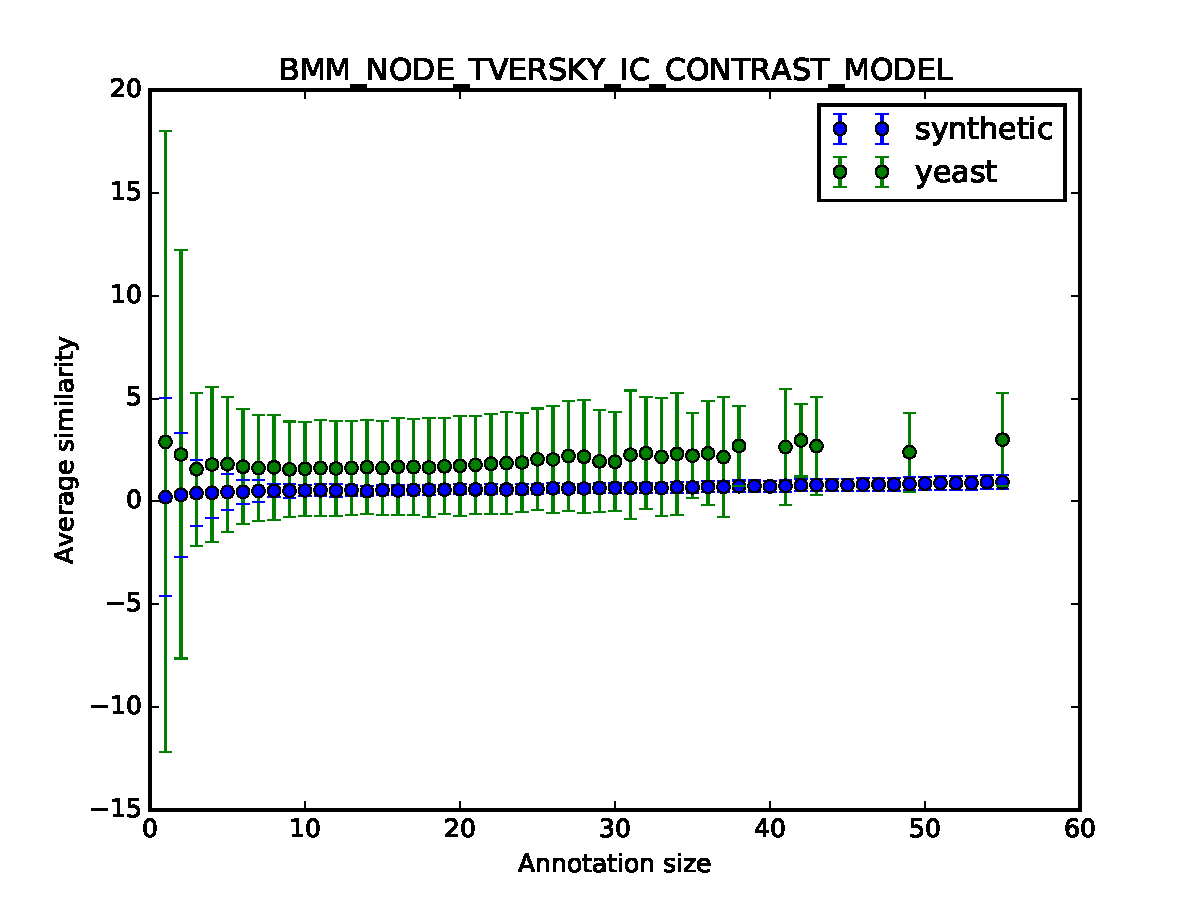
\includegraphics[width=0.5\linewidth, height=0.4\textheight]{pairwise/SIM_GROUPWISE_BMM_SIM_PAIRWISE_DAG_NODE_TVERSKY_IC_CONTRAST_MODEL_avg.pdf}
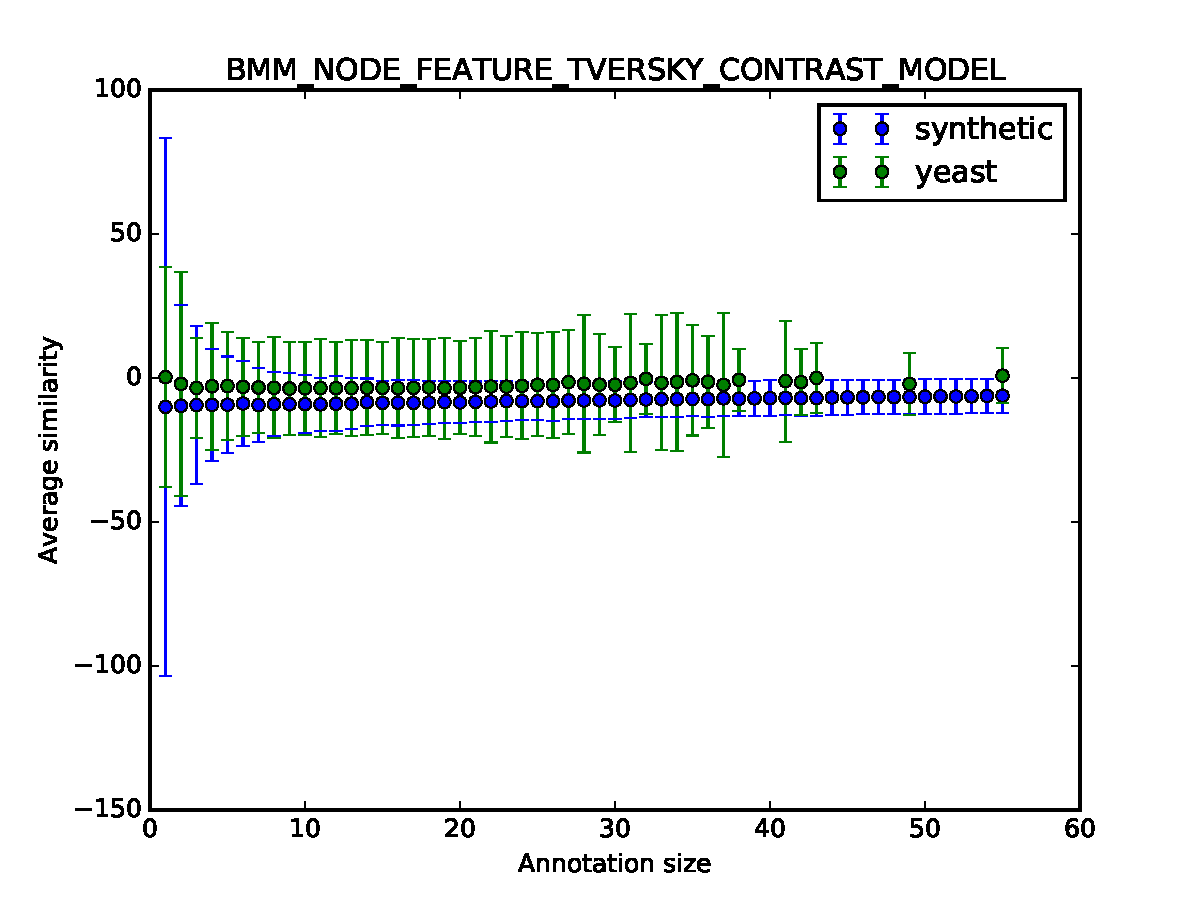
\includegraphics[width=0.5\linewidth, height=0.4\textheight]{pairwise/SIM_GROUPWISE_BMM_SIM_PAIRWISE_DAG_NODE_FEATURE_TVERSKY_CONTRAST_MODEL_avg.pdf}
\end{figure}
\end{frame}


\begin{frame}{Groupwise Similarity Measures}
\begin{figure}
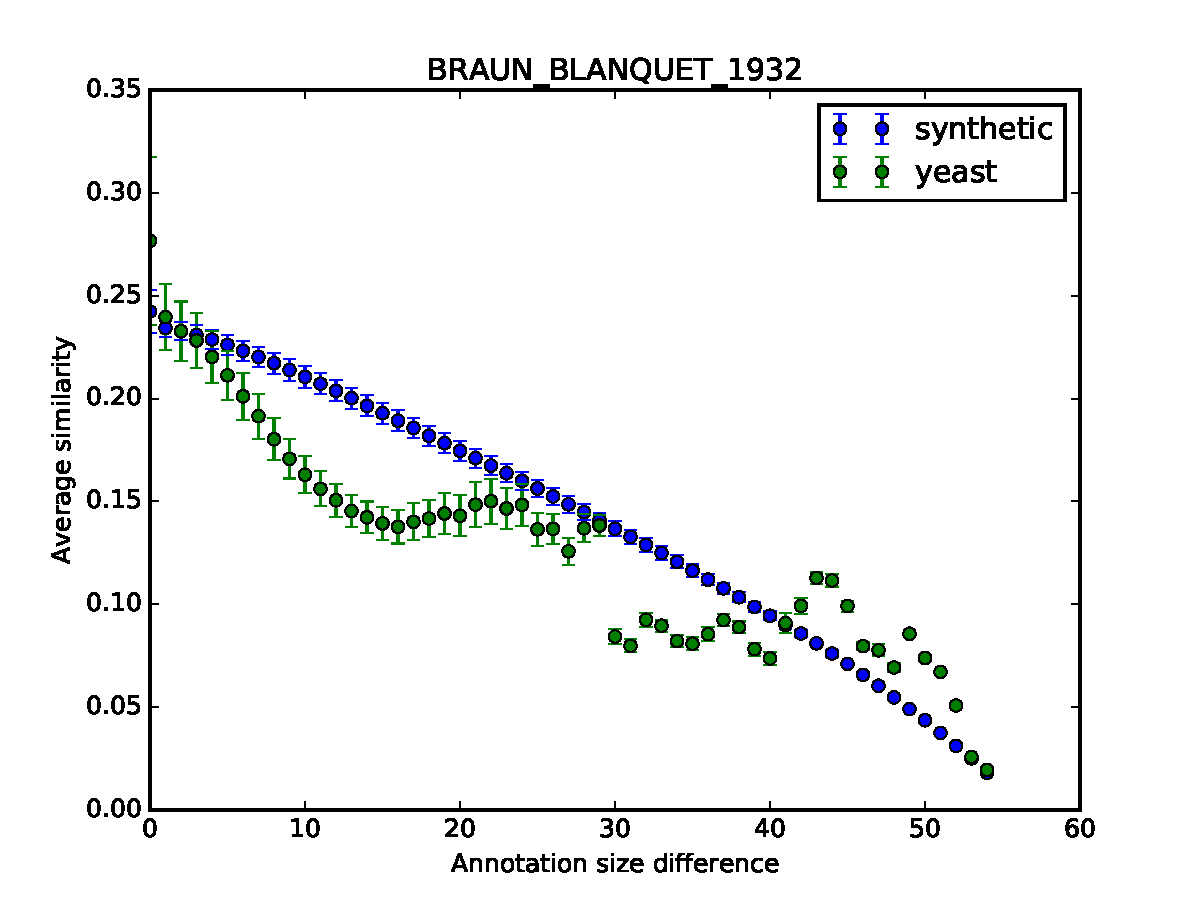
\includegraphics[width=0.5\linewidth, height=0.4\textheight]{groupwise_diff/SIM_FRAMEWORK_DAG_SET_BRAUN_BLANQUET_1932_diff.pdf}
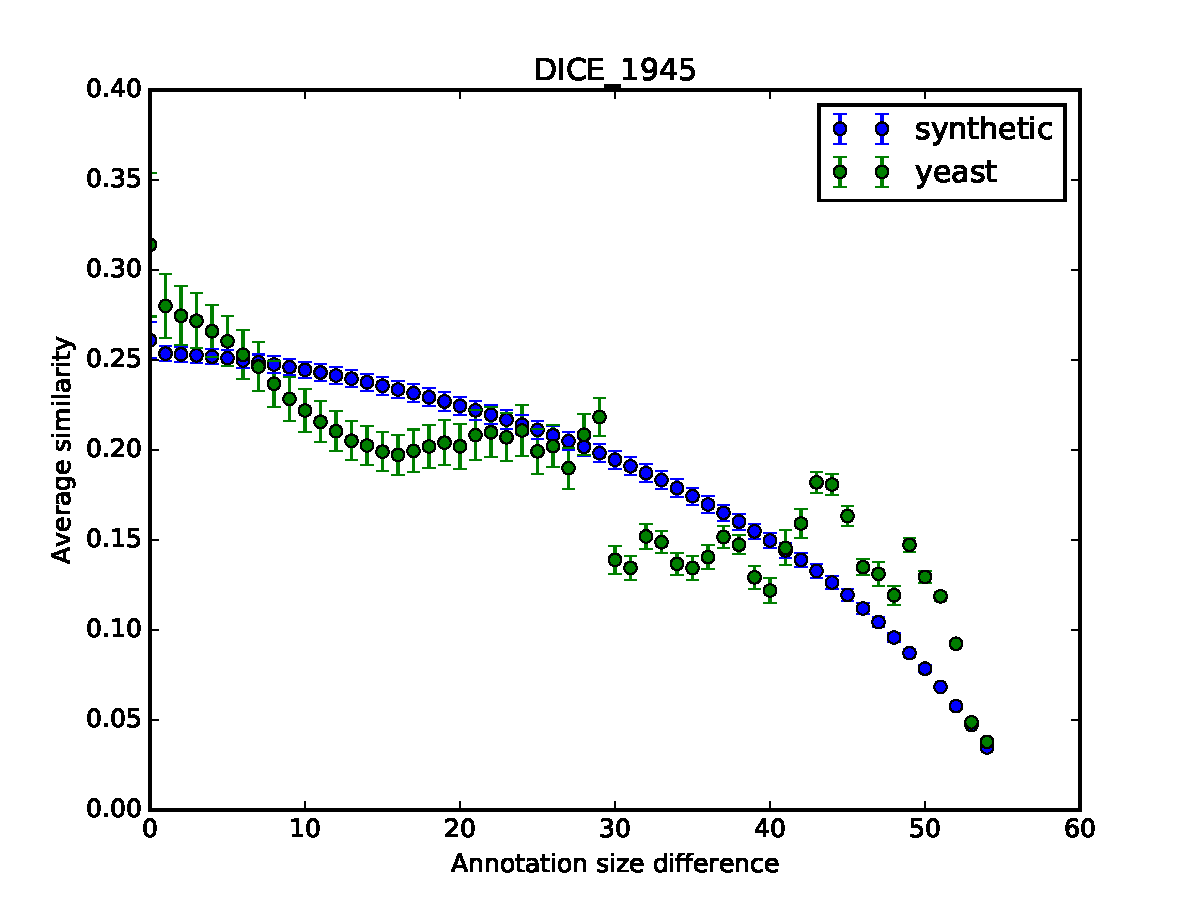
\includegraphics[width=0.5\linewidth, height=0.4\textheight]{groupwise_diff/SIM_FRAMEWORK_DAG_SET_DICE_1945_diff.pdf} \\
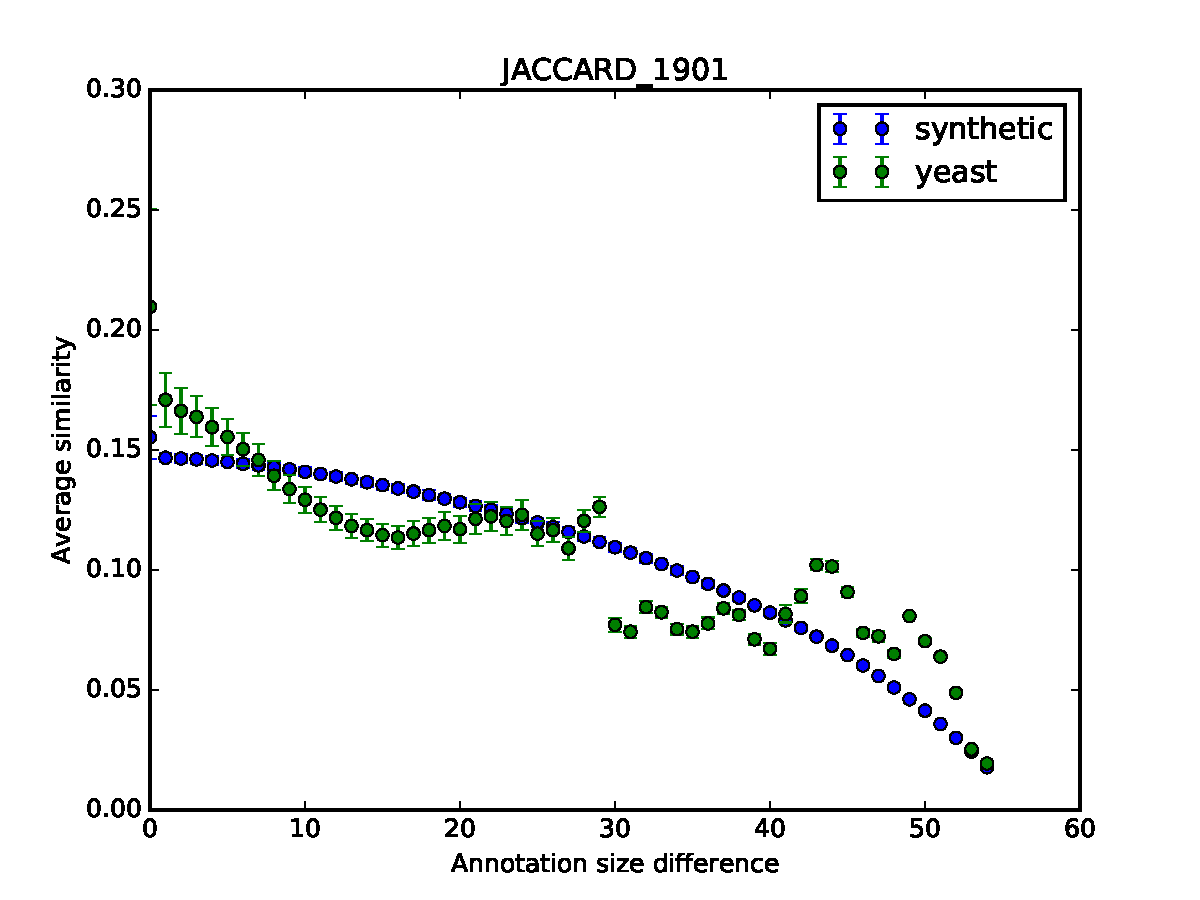
\includegraphics[width=0.5\linewidth, height=0.4\textheight]{groupwise_diff/SIM_FRAMEWORK_DAG_SET_JACCARD_1901_diff.pdf}
\includegraphics[width=0.5\linewidth, height=0.4\textheight]{groupwise_diff/SIM_GROUPWISE_DAG_GIC_diff.pdf}
\end{figure}
\end{frame}

\begin{frame}{Groupwise Similarity Measures}
\begin{figure}
\includegraphics[width=0.5\linewidth, height=0.4\textheight]{groupwise_diff/SIM_FRAMEWORK_DAG_SET_KNAPPE_2004_diff.pdf}
\includegraphics[width=0.5\linewidth, height=0.4\textheight]{groupwise_diff/SIM_FRAMEWORK_DAG_SET_KORBEL_2002_diff.pdf} \\
\includegraphics[width=0.5\linewidth, height=0.4\textheight]{groupwise_diff/SIM_FRAMEWORK_DAG_SET_SIMPSON_1960_diff.pdf}
\includegraphics[width=0.5\linewidth, height=0.4\textheight]{groupwise_diff/SIM_GROUPWISE_DAG_NTO_diff.pdf}
\end{figure}
\end{frame}

\begin{frame}{Groupwise Similarity Measures}
\begin{figure}
\includegraphics[width=0.5\linewidth, height=0.4\textheight]{groupwise_diff/SIM_GROUPWISE_DAG_LEE_2004_diff.pdf}
\includegraphics[width=0.5\linewidth, height=0.4\textheight]{groupwise_diff/SIM_GROUPWISE_DAG_TO_diff.pdf} \end{figure}
\end{frame}


\begin{frame}{Pairwise Similarity Measures}
\begin{figure}
\includegraphics[width=0.5\linewidth, height=0.4\textheight]{pairwise_diff/SIM_GROUPWISE_AVERAGE_NORMALIZED_GOSIM_SIM_PAIRWISE_DAG_NODE_LIN_1998_diff.pdf}
\includegraphics[width=0.5\linewidth, height=0.4\textheight]{pairwise_diff/SIM_GROUPWISE_AVERAGE_NORMALIZED_GOSIM_SIM_PAIRWISE_DAG_NODE_RESNIK_1995_diff.pdf} \\
\includegraphics[width=0.5\linewidth, height=0.4\textheight]{pairwise_diff/SIM_GROUPWISE_AVERAGE_NORMALIZED_GOSIM_SIM_PAIRWISE_DAG_NODE_SCHLICKER_2006_diff.pdf}
\includegraphics[width=0.5\linewidth, height=0.4\textheight]{pairwise_diff/SIM_GROUPWISE_AVERAGE_NORMALIZED_GOSIM_SIM_PAIRWISE_DAG_NODE_SCHLICKER_JACCARD_diff.pdf}
\end{figure}
\end{frame}

\begin{frame}{Pairwise Similarity Measures}
\begin{figure}
\includegraphics[width=0.5\linewidth, height=0.4\textheight]{pairwise_diff/SIM_GROUPWISE_AVERAGE_NORMALIZED_GOSIM_SIM_PAIRWISE_DAG_NODE_LIN_1998_diff.pdf}
\includegraphics[width=0.5\linewidth, height=0.4\textheight]{pairwise_diff/SIM_GROUPWISE_AVERAGE_NORMALIZED_GOSIM_SIM_PAIRWISE_DAG_NODE_RESNIK_1995_diff.pdf} \\
\includegraphics[width=0.5\linewidth, height=0.4\textheight]{pairwise_diff/SIM_GROUPWISE_AVERAGE_NORMALIZED_GOSIM_SIM_PAIRWISE_DAG_NODE_SCHLICKER_2006_diff.pdf}
\includegraphics[width=0.5\linewidth, height=0.4\textheight]{pairwise_diff/SIM_GROUPWISE_AVERAGE_NORMALIZED_GOSIM_SIM_PAIRWISE_DAG_NODE_SCHLICKER_JACCARD_diff.pdf}
\end{figure}
\end{frame}
%-----------------------------------------------

\begin{frame}
\frametitle{References}
\footnotesize{
\begin{thebibliography}{99} % Beamer does not support BibTeX so references must be inserted manually as below
\bibitem[Harispe, 2015]{p1} Sebastien Harispe*, Sylvie Ranwez, Stefan Janaqi and Jacky Montmain (2015)
\newblock Semantic Similarity from Natural Language and Ontology Analysis  
\newblock \emph{Synthesis Lectures on Human Language Technologies
} Vol. 8, No. 1 , Pages 1-254.
\bibitem[Harispe]{p2} Semantic Measures Library owned by Sebastien Harispe, http://www.semantic-measures-library.org/
\end{thebibliography}
}
\end{frame}

%------------------------------------------------

\begin{frame}
\Huge{\centerline{Thanks!}}
\end{frame}

%----------------------------------------------------------------------------------------

\end{document}